% Document Structure
\documentclass[12pt, oneside]{book}
\usepackage{geometry} % 1 inch margins

% Encoding
\usepackage[T1]{fontenc}

% Color
\usepackage[table,xcdraw,dvipsnames]{xcolor}

% Table of Contents and Lists
\setcounter{secnumdepth}{3} % fuck it, subsubsection numbers 
\setcounter{tocdepth}{3} % might as well put them in the ToC too!
\usepackage[nottoc]{tocbibind} % don't list ToC itself in ToC
\usepackage[titles]{tocloft}
\cftsetindents{figure}{0em}{1.5em}
\setcounter{lofdepth}{2} % list subfigures in LoF

% \renewcommand{\cftchapleader}{\cftdotfill{\cftdotsep}} % dotted line for all depths

% typefaces
\usepackage{lmodern}
\usepackage[tt=false,oldstyle,proportional,semibold]{libertine}
\usepackage{libertinust1math}

% highlight boxes
\usepackage[most]{tcolorbox} 
    % multiline highlight
    \definecolor{light-gray}{gray}{0.9}
    \tcbset{
        on line, boxsep=3pt, left=0pt,right=0pt,top=0pt,bottom=-1pt, colframe=white,colback=light-gray, highlight math style={enhanced}
    }

    % Sans serif grey highlight for software tools
    \newcommand{\hltt}[1]{\tcbox{\vphantom{lg}\texttt{#1}}}

    % typewriter grey highlight for code
    \newcommand{\hlss}[1]{\tcbox{\vphantom{lg}{\sffamily{#1}}}}

% Justification
\usepackage[nopatch=footnote]{microtype} % small adjustments
\usepackage{indentfirst} % paragraphs

% vertical spacing
\usepackage{setspace}
\setstretch{1.5}

% Page Header & Footer
\usepackage[twoside]{fancyhdr}

% custom running header
\makeatletter % use @ as letter character
\renewcommand{\chaptermark}[1]{\markboth{\ifnum\value{chapter}=0\else\@chapapp~\thechapter: \fi #1}{}} % don't show chapter number in header if 0 (frontmatter lists)
\makeatother % protect @ character

\setlength{\headheight}{15pt}
\addtolength{\topmargin}{-2.5pt}
\usepackage{appendix}

\newcommand\MakeMarkcase{} % remove \MakeUppercase (replace with small caps below)


% custom page header
\AtBeginDocument{
    \pagestyle{fancy}
    \fancyhead{} % clear all header fields
    \fancyhead[RE,LO]{\textsc\leftmark} % chapter outer upper corner
    \fancyfoot{} % clear all footer fields
    \fancyfoot[C]{\thepage} % page number center bottom
}

% Chapter Header with box 
\usepackage{titlesec}
\titleformat{\chapter}[frame]
{\normalfont}{\filright\fbox{\enspace%
{\textsc{\chaptertitlename~\thechapter}}\enspace}}{8pt}{\Large\bfseries\filcenter}

% table of contents and list of figures (no MakeUpperCase nonsense)
\makeatletter
\renewcommand\tableofcontents{%
    \chapter*{\contentsname
        \@mkboth{%
           \contentsname}{\contentsname}}%
    \@starttoc{toc}%
}

\makeatother

% hack to make small caps header
\renewcommand\listfigurename{L\lowercase{ist of} F\lowercase{igures}}

% Footnotes
\usepackage[hang,splitrule,multiple]{footmisc}
\setlength{\footnotemargin}{1em}
\interfootnotelinepenalty=10000


% Internal References
\usepackage{hyperref}
\hypersetup{pdfborder = {0 0 0}} % no boxes around links
\usepackage[all]{hypcap} % link to figure (not caption)

% Continuous numbering (not by section)
\usepackage{chngcntr}
\counterwithout{figure}{chapter}
\counterwithout{table}{chapter}
\counterwithout{equation}{chapter}

% Lists
\usepackage{paralist} % inline lists
\usepackage[inline]{enumitem}
\setlist[itemize]{noitemsep,nolistsep}
\setlist[enumerate]{noitemsep,nolistsep}

% Technical
\usepackage{amsmath}
\renewcommand\theequation{\liningnums{\arabic{equation}}} % use full height (not old style) numbers for equation tags
\usepackage[separate-uncertainty=true]{siunitx}
\usepackage{wasysym}

\usepackage{adjustbox}
\usepackage{multirow}
\usepackage[labelfont={bf}]{caption} % captions
\usepackage[listformat=simple]{subcaption} % figure subparts [would love to have list=true here without extremely deep indents]

% Abbreviations
\usepackage{supertabular}
\usepackage{tabularray}
\DefTblrTemplate{caption-tag}{normal}{}
\SetTblrTemplate{caption-tag}{normal}
\DefTblrTemplate{caption-sep}{normal}{}
\SetTblrTemplate{caption-sep}{normal}
\DefTblrTemplate{conthead-text}{normal}{}
\SetTblrTemplate{conthead-text}{normal}

% vertically align perfectly with textwidth
\DefTblrTemplate{width}{normal}{1.1\textwidth}
\SetTblrTemplate{width}{normal}

\usepackage{acro}
\acsetup{make-links=true}
% customize list format with an extra column for alt (code)
\DeclareAcroProperty{code}

\DeclareAcronym{MOLA}{
  short=MOLA,
  long=Mars Orbiter Laser Altimeter,
}
\DeclareAcronym{CTX}{
  short=CTX,
  long=Context Camera,
}
\DeclareAcronym{MRO}{
  short=MRO,
  long=Mars Reconnaissance Orbiter,
}
\DeclareAcronym{MGS}{
  short=MGS,
  long=Mars Global Surveyor,
}
\DeclareAcronym{HRSC}{
  short=HRSC,
  long=High-Resolution Stereo Camera,
}
\DeclareAcronym{ESA}{
  short=ESA,
  long=European Space Agency,
}
\DeclareAcronym{NASA}{
  short=NASA,
  long=National Aeronautics and Space Administration,
  first-style=short
}
\DeclareAcronym{MEX}{
  short=MEX,
  long=Mars Express,
}
\DeclareAcronym{DEM}{
  short=DEM,
  long=digital elevation model,
}
\DeclareAcronym{LIP}{
  short=LIP,
  long=Large Igneous Province,
}

\DeclareAcronym{LHB}{
  short=LHB,
  long=Late Heavy Bombardment,
}
\DeclareAcronym{FEM}{
  short=FEM,
  long=finite element method,
}
\DeclareAcronym{RMSE}{
  short=RMSE,
  long=root mean square error,
}
\DeclareAcronym{lat}{
  short = \ensuremath{\delta_S},
  long = latitude of sample,
  tag = sym,
  code = lat1
}

\DeclareAcronym{lon}{
  short = \ensuremath{\lambda_S},
  long = longitude of sample,
  tag = sym,
  code = lon1
}

\DeclareAcronym{latC}{
  short = \ensuremath{\delta_C},
  long = latitude of center,
  tag = sym,
  code = lat2
}

\DeclareAcronym{lonC}{
  short = \ensuremath{\lambda_C},
  long = longitude of center,
  tag = sym,
  code = lon2
}

\DeclareAcronym{az1}{
  short = \ensuremath{\theta_1},
  long = paleo-azimuth,
  tag = sym,
  code = az1
}

\DeclareAcronym{sl1}{
  short = \ensuremath{\varphi_1},
  long = paleo-slope,
  tag = sym,
  code = sl1
}

\DeclareAcronym{az2}{
  short = \ensuremath{\theta_2},
  long = azimuth,
  tag = sym,
  code = az2
}

\DeclareAcronym{sl2}{
  short = \ensuremath{\varphi_2},
  long = slope,
  tag = sym,
  code = sl2
}

\DeclareAcronym{disc}{
  short = \ensuremath{\Delta\theta},
  long = topographic discordance,
  tag = sym,
}

\DeclareAcronym{center}{
  short = \ensuremath{C},
  long = candidate axisymmetric center point,
  tag = sym
}

\DeclareAcronym{bearing}{
  short = \ensuremath{\Theta},
  long = bearing from sample away from center,
  tag = sym,
  code = theta
}

\DeclareAcronym{dist}{
  short = \ensuremath{r},
  long = radial distance,
  tag = sym,
  code = dist
}

\DeclareAcronym{normal2}{
  short = \ensuremath{\vec{n}_2},
  long = pole to modern topographic surface plane,
  tag = sym
}

\DeclareAcronym{normal1}{
  short = \ensuremath{\vec{n}_1},
  long = pole to estimated paleo-surface plane,
  tag = sym
}

\DeclareAcronym{axsl2}{
  short = \ensuremath{\Phi_2},
  long = slope of displaced model surface,
  tag = sym
}

\DeclareAcronym{axsl1}{
  short = \ensuremath{\Phi_1},
  long = slope of initial model surface,
  tag = sym
}

\DeclareAcronym{tilt}{
  short = \ensuremath{\Phi},
  long = tilt,
  tag = sym,
  code = tilt
}

\DeclareAcronym{tilt_min}{
  short = \ensuremath{\alpha},
  long = minimum tilt,
  tag = sym,
  code = tilt\_min
}

\DeclareAcronym{north}{
  short = \textbf{N},
  long = north,
  tag = sym
}

\DeclareAcronym{disp_a}{
  short = \ensuremath{U_A},
  long = displacement of element node $A$ (proximal),
  tag = sym
}

\DeclareAcronym{disp_b}{
  short = \ensuremath{U_B},
  long = displacement of element node $B$ (distal),
  tag = sym
}

\DeclareAcronym{ddisp}{
  short = \ensuremath{\Delta U},
  long = $\acs{disp_b} - \acs{disp_a}$,
  tag = sym
}

\DeclareAcronym{disp}{
  short = \ensuremath{U},
  long = displacement,
  tag = sym,
  code = disp
}
\DeclareAcronym{disp_z}{
  short = \ensuremath{U_z},
  long = vertical component of \acs{disp},
  tag = sym,
  code = disp[1]
}
\DeclareAcronym{disp_r}{
  short = \ensuremath{U_r},
  long = radial component of \acs{disp},
  tag = sym,
  code = disp[0]
}

\DeclareAcronym{ddisp_z}{
  short = \ensuremath{\Delta U_z},
  long = vertical component of \acs{ddisp},
  tag = sym
}
\DeclareAcronym{ddisp_r}{
  short = \ensuremath{\Delta U_r},
  long = radial component of \acs{ddisp},
  tag = sym
}

\DeclareAcronym{disp_z'}{
  short = \ensuremath{U_z'},
  long = derivative of \acs{ddisp_z} with respect to $r_1$,
  tag = sym
}
\DeclareAcronym{disp_r'}{
  short = \ensuremath{U_r'},
  long = derivative of \acs{ddisp_r} with respect to $r_1$,
  tag = sym
}

\DeclareAcronym{z1'}{
  short = \ensuremath{z_1'},
  long = slope (essentially),
  tag = sym
}
\DeclareAcronym{dr1}{
  short = \ensuremath{\Delta r_1},
  long = radial distance between nodes $A$ and $B$,
  tag = sym
}
\DeclareAcronym{dz1}{
  short = \ensuremath{\Delta z_1},
  long = vertical distance between nodes $A$ and $B$,
  tag = sym
}
\DeclareAcronym{DtT}{
  short = \ensuremath{DtT},
  long = depth to top of magma reservoir,
  tag = sym,
  code = DtT
}
\DeclareAcronym{Rr}{
  short = \ensuremath{resr},
  long = magma reservoir radial (horizontal) radius,
  tag = sym,
  code = resr
}
\DeclareAcronym{Rz}{
  short = \ensuremath{resz},
  long = magma reservoir vertical radius,
  tag = sym,
  code = resz
}
\DeclareAcronym{g}{
  short = \ensuremath{g},
  long = gravity of Mars,
  tag = sym,
}
\DeclareAcronym{mult}{
  short = \ensuremath{pmult},
  long = multiplier for over- or underpressure,
  tag = sym,
  code = pmult
}
\DeclareAcronym{rhor}{
  short = \ensuremath{\rho_\text{rock}},
  long = rock density,
  tag = sym,
  code = rhor
}
\DeclareAcronym{dP}{
  short = \ensuremath{\Delta P},
  long = over- (positive) or under- (negative) pressure,
  tag = sym,
  code = dP
}
\DeclareAcronym{beta1}{
  short = \ensuremath{\beta_1},
  long = \ensuremath{\acs{az1}-\acs{bearing}},
  tag = sym,
  code = beta1
}
\DeclareAcronym{beta2}{
  short = \ensuremath{\beta_2},
  long = \ensuremath{\acs{az2}-\acs{bearing}},
  tag = sym,
  code = beta2
}

\DeclareAcronym{epv}{
  short = \ensuremath{E_{PV}},
  long = inflation energy,
  tag = sym,
  code = epv
}

\DeclareAcronym{depth}{
  short = \ensuremath{d},
  long = depth to center of reservoir,
  tag = sym,
  code = d
}

% \RenewAcroTemplate [list] {tabularray}
%   {
%     \AcroNeedPackage {tabularray}
%     \acronymsmapF
%       {
%         \AcroAddRow
%           {
%             \acrowrite {short}
%             & 
%             \acroifT{code}{\hltt{\acrowrite{code}}}
%             &
%             \acrowrite {list}
%             \acroifanyT {foreign,extra} {~(}
%             \acrowrite {foreign}
%             \acroifallT {foreign,extra} {,~}
%             \acrowrite {extra}
%             \acroifanyT {foreign,extra} {)}
%             \acropagefill
%             \acropages
%               { \acrotranslate {page} \nobreakspace }
%               { \acrotranslate {pages} \nobreakspace }
%             \strut \\
%           }
%       }
%       { \AcroRerun }
%     \acroheading
%     \acropreamble
%     \par \noindent
%     \begin{actblr}{
%         column{1} = {leftsep=-2pt},
%         column{3} = {rightsep=-2pt},
%         width=\textwidth,
%         colspec = {llX[l]},
%         column{1} = { font = \bfseries }
%         }
%       \AcronymTable
%     \end{actblr}
%   }

% GSA Citations & Bibliography
% Package
\usepackage[giveninits=true,uniquename=init,backend=biber,style=authoryear,maxbibnames=10]{biblatex}
\usepackage{xpatch} % I'm stuff

\setlength{\bibhang}{2em} % hanging indent length 

% ``Referenced Cited'' Section Title 
\AtBeginDocument{\renewcommand{\bibname}{References Cited}}

% change header mark 
\DefineBibliographyStrings{english}{%
  references = {\textsc{References Cited}}
}

% Sources
\addbibresource{aux/references.bib}

% Punctuation
\renewcommand*{\nameyeardelim}{\addcomma\space}
\renewcommand*{\newunitpunct}{\addcomma\space}

% don't print these fields. for some reason, language still prints, so make sure it is missing from each entry in the .bib file.
\AtEveryBibitem{
  \clearfield{address}
  \clearfield{url}
  \clearfield{urlyear}
  \clearfield{urlmonth}
  \clearfield{issn}
  \clearfield{month}
  \clearfield{day}
  \clearfield{note}
  \clearfield{series}
  \clearfield{language}
}

% Surname, [Initials] for ALL authors
\DeclareNameAlias{sortname}{family-given}

% thin space between author initials
\renewrobustcmd*{\bibinitdelim}{\hspace{1pt}}

% remove parentheses from bibliography dates
\xpatchbibmacro{date+extradate}{\printtext[parens]}{\newunit\printtext}{}{}

% Plain format for title & journal
\DeclareFieldFormat*{title}{#1}
\DeclareFieldFormat*{journaltitle}{#1}

% replace `in:' before journal with `:'
\renewbibmacro{in:}{}
\xpatchbibdriver{article}
  {\usebibmacro{title}\newunit}
  {\usebibmacro{title}\printunit{\addcolon\space}}{}{}

% Journal Volume, Number
\DeclareFieldFormat*{volume}{v. #1}
\DeclareFieldFormat*{number}{no. #1}

% comma between Volume and Number
\renewbibmacro*{volume+number+eid}{%
  \newunit
  \printfield{volume}%
  \newunit
  \printfield{number}%
  }

% p. (not pp.)
\DefineBibliographyStrings{english}{pages = {p.},}

% Hyperlink DOI
\DeclareFieldFormat*{doi}{\href{http://dx.doi.org/\thefield{doi}}{doi:#1}}

% Figures & Tables
\usepackage{floatrow} % figures with side captions

% Graphics
\usepackage{graphicx} % include images
\graphicspath{{figures/}} % image location

% settings and variables defined 
\usepackage{tikz}
\usetikzlibrary{shapes, arrows, positioning}
\tikzstyle{arrow} = [very thick, -latex]
\tikzstyle{axis} = [semithick, -latex]

\usepackage{tikz-3dplot}

% figure view angle
\pgfmathsetmacro{\viewze}{65}
\pgfmathsetmacro{\viewaz}{107}
\tdplotsetmaincoords{\viewze}{\viewaz}

% define lengths
\pgfmathsetmacro{\radius}{1.3}
\pgfmathsetmacro{\axislength}{1.4}

% define angles for (az2, sl2) pole 
\pgfmathsetmacro{\az}{40}
\pgfmathsetmacro{\ze}{37}

% define angles (az1, az1) plane and pole
\pgfmathsetmacro{\azi}{0}
\pgfmathsetmacro{\zen}{18.676174754207974} % calculated
\pgfmathsetmacro{\sinzen}{0.3202190853902431} % calculated

% define az for reversal
\pgfmathsetmacro{\azrev}{2*\azi+180-\az}

% optimize cenang
\pgfmathsetmacro{\cenang}{34.438487775} % calculated

% define radial projection azimuth
\pgfmathsetmacro{\THETA}{70}

% ze_project (all calculated)
\pgfmathsetmacro{\zeproj}{33.128344027484886}
\pgfmathsetmacro{\zenproj}{6.594628182428004}

\pgfmathsetmacro{\deltalength}{.3009075*\radius}
\pgfmathsetmacro{\asindelta}{-17.512118517810134}
\pgfmathsetmacro{\smallcircleradius}{0.953653327722986*\radius}

\pgfmathsetmacro{\poleoneflatx}{0.3261686478308167*\smallcircleradius}
\pgfmathsetmacro{\poletwoflatx}{0.8258880082116726*\smallcircleradius}

\newcommand{\flatradius}{2.5}%
\newcommand{\uncert}{25}%

% use jupyter tex output (body, no figures)
\usepackage{amssymb} % Equations
\usepackage{textcomp} % defines textquotesingle
% Hack from http://tex.stackexchange.com/a/47451/13684:
\AtBeginDocument{%
    \def\PYZsq{\textquotesingle}% Upright quotes in Pygmentized code
}
\usepackage{upquote} % Upright quotes for verbatim code
\usepackage{eurosym} % defines \euro

\usepackage{iftex}
\ifPDFTeX
    \usepackage[T1]{fontenc}
    \IfFileExists{alphabeta.sty}{
          \usepackage{alphabeta}
      }{
          \usepackage[mathletters]{ucs}
          \usepackage[utf8x]{inputenc}
      }
\else
    \usepackage{fontspec}
    \usepackage{unicode-math}
\fi

\usepackage{fancyvrb} % verbatim replacement that allows latex
\usepackage{grffile} % extends the file name processing of package graphics
                     % to support a larger range
\makeatletter % fix for old versions of grffile with XeLaTeX
\@ifpackagelater{grffile}{2019/11/01}
{
  % Do nothing on new versions
}
{
  \def\Gread@@xetex#1{%
    \IfFileExists{"\Gin@base".bb}%
    {\Gread@eps{\Gin@base.bb}}%
    {\Gread@@xetex@aux#1}%
  }
}
\makeatother


\usepackage{longtable} % longtable support required by pandoc >1.10
\usepackage{booktabs}  % table support for pandoc > 1.12.2
\usepackage{array}     % table support for pandoc >= 2.11.3
\usepackage{calc}      % table minipage width calculation for pandoc >= 2.11.1

\usepackage[normalem]{ulem} % ulem is needed to support strikethroughs (\sout)
                            % normalem makes italics be italics, not underlines
\usepackage{mathrsfs}



% Colors for the hyperref package
\definecolor{urlcolor}{rgb}{0,.145,.698}
\definecolor{linkcolor}{rgb}{.71,0.21,0.01}
\definecolor{citecolor}{rgb}{.12,.54,.11}

% ANSI colors
\definecolor{ansi-black}{HTML}{3E424D}
\definecolor{ansi-black-intense}{HTML}{282C36}
\definecolor{ansi-red}{HTML}{E75C58}
\definecolor{ansi-red-intense}{HTML}{B22B31}
\definecolor{ansi-green}{HTML}{00A250}
\definecolor{ansi-green-intense}{HTML}{007427}
\definecolor{ansi-yellow}{HTML}{DDB62B}
\definecolor{ansi-yellow-intense}{HTML}{B27D12}
\definecolor{ansi-blue}{HTML}{208FFB}
\definecolor{ansi-blue-intense}{HTML}{0065CA}
\definecolor{ansi-magenta}{HTML}{D160C4}
\definecolor{ansi-magenta-intense}{HTML}{A03196}
\definecolor{ansi-cyan}{HTML}{60C6C8}
\definecolor{ansi-cyan-intense}{HTML}{258F8F}
\definecolor{ansi-white}{HTML}{C5C1B4}
\definecolor{ansi-white-intense}{HTML}{A1A6B2}
\definecolor{ansi-default-inverse-fg}{HTML}{FFFFFF}
\definecolor{ansi-default-inverse-bg}{HTML}{000000}

% common color for the border for error outputs.
\definecolor{outerrorbackground}{HTML}{FFDFDF}

% commands and environments needed by pandoc snippets
% extracted from the output of `pandoc -s`
\providecommand{\tightlist}{%
  \setlength{\itemsep}{0pt}\setlength{\parskip}{0pt}}
\DefineVerbatimEnvironment{Highlighting}{Verbatim}{commandchars=\\\{\}}
% Add ',fontsize=\small' for more characters per line
\newenvironment{Shaded}{}{}
\newcommand{\KeywordTok}[1]{\textcolor[rgb]{0.00,0.44,0.13}{\textbf{{#1}}}}
\newcommand{\DataTypeTok}[1]{\textcolor[rgb]{0.56,0.13,0.00}{{#1}}}
\newcommand{\DecValTok}[1]{\textcolor[rgb]{0.25,0.63,0.44}{{#1}}}
\newcommand{\BaseNTok}[1]{\textcolor[rgb]{0.25,0.63,0.44}{{#1}}}
\newcommand{\FloatTok}[1]{\textcolor[rgb]{0.25,0.63,0.44}{{#1}}}
\newcommand{\CharTok}[1]{\textcolor[rgb]{0.25,0.44,0.63}{{#1}}}
\newcommand{\StringTok}[1]{\textcolor[rgb]{0.25,0.44,0.63}{{#1}}}
\newcommand{\CommentTok}[1]{\textcolor[rgb]{0.38,0.63,0.69}{\textit{{#1}}}}
\newcommand{\OtherTok}[1]{\textcolor[rgb]{0.00,0.44,0.13}{{#1}}}
\newcommand{\AlertTok}[1]{\textcolor[rgb]{1.00,0.00,0.00}{\textbf{{#1}}}}
\newcommand{\FunctionTok}[1]{\textcolor[rgb]{0.02,0.16,0.49}{{#1}}}
\newcommand{\RegionMarkerTok}[1]{{#1}}
\newcommand{\ErrorTok}[1]{\textcolor[rgb]{1.00,0.00,0.00}{\textbf{{#1}}}}
\newcommand{\NormalTok}[1]{{#1}}

% Additional commands for more recent versions of Pandoc
\newcommand{\ConstantTok}[1]{\textcolor[rgb]{0.53,0.00,0.00}{{#1}}}
\newcommand{\SpecialCharTok}[1]{\textcolor[rgb]{0.25,0.44,0.63}{{#1}}}
\newcommand{\VerbatimStringTok}[1]{\textcolor[rgb]{0.25,0.44,0.63}{{#1}}}
\newcommand{\SpecialStringTok}[1]{\textcolor[rgb]{0.73,0.40,0.53}{{#1}}}
\newcommand{\ImportTok}[1]{{#1}}
\newcommand{\DocumentationTok}[1]{\textcolor[rgb]{0.73,0.13,0.13}{\textit{{#1}}}}
\newcommand{\AnnotationTok}[1]{\textcolor[rgb]{0.38,0.63,0.69}{\textbf{\textit{{#1}}}}}
\newcommand{\CommentVarTok}[1]{\textcolor[rgb]{0.38,0.63,0.69}{\textbf{\textit{{#1}}}}}
\newcommand{\VariableTok}[1]{\textcolor[rgb]{0.10,0.09,0.49}{{#1}}}
\newcommand{\ControlFlowTok}[1]{\textcolor[rgb]{0.00,0.44,0.13}{\textbf{{#1}}}}
\newcommand{\OperatorTok}[1]{\textcolor[rgb]{0.40,0.40,0.40}{{#1}}}
\newcommand{\BuiltInTok}[1]{{#1}}
\newcommand{\ExtensionTok}[1]{{#1}}
\newcommand{\PreprocessorTok}[1]{\textcolor[rgb]{0.74,0.48,0.00}{{#1}}}
\newcommand{\AttributeTok}[1]{\textcolor[rgb]{0.49,0.56,0.16}{{#1}}}
\newcommand{\InformationTok}[1]{\textcolor[rgb]{0.38,0.63,0.69}{\textbf{\textit{{#1}}}}}
\newcommand{\WarningTok}[1]{\textcolor[rgb]{0.38,0.63,0.69}{\textbf{\textit{{#1}}}}}


% Define a nice break command that doesn't care if a line doesn't already
% exist.
\def\br{\hspace*{\fill} \\* }
% Math Jax compatibility definitions
\def\gt{>}
\def\lt{<}
\let\Oldtex\TeX
\let\Oldlatex\LaTeX
\renewcommand{\TeX}{\textrm{\Oldtex}}
\renewcommand{\LaTeX}{\textrm{\Oldlatex}}
% Document parameters
% Document title
\title{code}





% Pygments definitions
\makeatletter
\def\PY@reset{\let\PY@it=\relax \let\PY@bf=\relax%
\let\PY@ul=\relax \let\PY@tc=\relax%
\let\PY@bc=\relax \let\PY@ff=\relax}
\def\PY@tok#1{\csname PY@tok@#1\endcsname}
\def\PY@toks#1+{\ifx\relax#1\empty\else%
\PY@tok{#1}\expandafter\PY@toks\fi}
\def\PY@do#1{\PY@bc{\PY@tc{\PY@ul{%
\PY@it{\PY@bf{\PY@ff{#1}}}}}}}
\def\PY#1#2{\PY@reset\PY@toks#1+\relax+\PY@do{#2}}

\@namedef{PY@tok@w}{\def\PY@tc##1{\textcolor[rgb]{0.73,0.73,0.73}{##1}}}
\@namedef{PY@tok@c}{\let\PY@it=\textit\def\PY@tc##1{\textcolor[rgb]{0.24,0.48,0.48}{##1}}}
\@namedef{PY@tok@cp}{\def\PY@tc##1{\textcolor[rgb]{0.61,0.40,0.00}{##1}}}
\@namedef{PY@tok@k}{\let\PY@bf=\textbf\def\PY@tc##1{\textcolor[rgb]{0.00,0.50,0.00}{##1}}}
\@namedef{PY@tok@kp}{\def\PY@tc##1{\textcolor[rgb]{0.00,0.50,0.00}{##1}}}
\@namedef{PY@tok@kt}{\def\PY@tc##1{\textcolor[rgb]{0.69,0.00,0.25}{##1}}}
\@namedef{PY@tok@o}{\def\PY@tc##1{\textcolor[rgb]{0.40,0.40,0.40}{##1}}}
\@namedef{PY@tok@ow}{\let\PY@bf=\textbf\def\PY@tc##1{\textcolor[rgb]{0.67,0.13,1.00}{##1}}}
\@namedef{PY@tok@nb}{\def\PY@tc##1{\textcolor[rgb]{0.00,0.50,0.00}{##1}}}
\@namedef{PY@tok@nf}{\def\PY@tc##1{\textcolor[rgb]{0.00,0.00,1.00}{##1}}}
\@namedef{PY@tok@nc}{\let\PY@bf=\textbf\def\PY@tc##1{\textcolor[rgb]{0.00,0.00,1.00}{##1}}}
\@namedef{PY@tok@nn}{\let\PY@bf=\textbf\def\PY@tc##1{\textcolor[rgb]{0.00,0.00,1.00}{##1}}}
\@namedef{PY@tok@ne}{\let\PY@bf=\textbf\def\PY@tc##1{\textcolor[rgb]{0.80,0.25,0.22}{##1}}}
\@namedef{PY@tok@nv}{\def\PY@tc##1{\textcolor[rgb]{0.10,0.09,0.49}{##1}}}
\@namedef{PY@tok@no}{\def\PY@tc##1{\textcolor[rgb]{0.53,0.00,0.00}{##1}}}
\@namedef{PY@tok@nl}{\def\PY@tc##1{\textcolor[rgb]{0.46,0.46,0.00}{##1}}}
\@namedef{PY@tok@ni}{\let\PY@bf=\textbf\def\PY@tc##1{\textcolor[rgb]{0.44,0.44,0.44}{##1}}}
\@namedef{PY@tok@na}{\def\PY@tc##1{\textcolor[rgb]{0.41,0.47,0.13}{##1}}}
\@namedef{PY@tok@nt}{\let\PY@bf=\textbf\def\PY@tc##1{\textcolor[rgb]{0.00,0.50,0.00}{##1}}}
\@namedef{PY@tok@nd}{\def\PY@tc##1{\textcolor[rgb]{0.67,0.13,1.00}{##1}}}
\@namedef{PY@tok@s}{\def\PY@tc##1{\textcolor[rgb]{0.73,0.13,0.13}{##1}}}
\@namedef{PY@tok@sd}{\let\PY@it=\textit\def\PY@tc##1{\textcolor[rgb]{0.73,0.13,0.13}{##1}}}
\@namedef{PY@tok@si}{\let\PY@bf=\textbf\def\PY@tc##1{\textcolor[rgb]{0.64,0.35,0.47}{##1}}}
\@namedef{PY@tok@se}{\let\PY@bf=\textbf\def\PY@tc##1{\textcolor[rgb]{0.67,0.36,0.12}{##1}}}
\@namedef{PY@tok@sr}{\def\PY@tc##1{\textcolor[rgb]{0.64,0.35,0.47}{##1}}}
\@namedef{PY@tok@ss}{\def\PY@tc##1{\textcolor[rgb]{0.10,0.09,0.49}{##1}}}
\@namedef{PY@tok@sx}{\def\PY@tc##1{\textcolor[rgb]{0.00,0.50,0.00}{##1}}}
\@namedef{PY@tok@m}{\def\PY@tc##1{\textcolor[rgb]{0.40,0.40,0.40}{##1}}}
\@namedef{PY@tok@gh}{\let\PY@bf=\textbf\def\PY@tc##1{\textcolor[rgb]{0.00,0.00,0.50}{##1}}}
\@namedef{PY@tok@gu}{\let\PY@bf=\textbf\def\PY@tc##1{\textcolor[rgb]{0.50,0.00,0.50}{##1}}}
\@namedef{PY@tok@gd}{\def\PY@tc##1{\textcolor[rgb]{0.63,0.00,0.00}{##1}}}
\@namedef{PY@tok@gi}{\def\PY@tc##1{\textcolor[rgb]{0.00,0.52,0.00}{##1}}}
\@namedef{PY@tok@gr}{\def\PY@tc##1{\textcolor[rgb]{0.89,0.00,0.00}{##1}}}
\@namedef{PY@tok@ge}{\let\PY@it=\textit}
\@namedef{PY@tok@gs}{\let\PY@bf=\textbf}
\@namedef{PY@tok@gp}{\let\PY@bf=\textbf\def\PY@tc##1{\textcolor[rgb]{0.00,0.00,0.50}{##1}}}
\@namedef{PY@tok@go}{\def\PY@tc##1{\textcolor[rgb]{0.44,0.44,0.44}{##1}}}
\@namedef{PY@tok@gt}{\def\PY@tc##1{\textcolor[rgb]{0.00,0.27,0.87}{##1}}}
\@namedef{PY@tok@err}{\def\PY@bc##1{{\setlength{\fboxsep}{\string -\fboxrule}\fcolorbox[rgb]{1.00,0.00,0.00}{1,1,1}{\strut ##1}}}}
\@namedef{PY@tok@kc}{\let\PY@bf=\textbf\def\PY@tc##1{\textcolor[rgb]{0.00,0.50,0.00}{##1}}}
\@namedef{PY@tok@kd}{\let\PY@bf=\textbf\def\PY@tc##1{\textcolor[rgb]{0.00,0.50,0.00}{##1}}}
\@namedef{PY@tok@kn}{\let\PY@bf=\textbf\def\PY@tc##1{\textcolor[rgb]{0.00,0.50,0.00}{##1}}}
\@namedef{PY@tok@kr}{\let\PY@bf=\textbf\def\PY@tc##1{\textcolor[rgb]{0.00,0.50,0.00}{##1}}}
\@namedef{PY@tok@bp}{\def\PY@tc##1{\textcolor[rgb]{0.00,0.50,0.00}{##1}}}
\@namedef{PY@tok@fm}{\def\PY@tc##1{\textcolor[rgb]{0.00,0.00,1.00}{##1}}}
\@namedef{PY@tok@vc}{\def\PY@tc##1{\textcolor[rgb]{0.10,0.09,0.49}{##1}}}
\@namedef{PY@tok@vg}{\def\PY@tc##1{\textcolor[rgb]{0.10,0.09,0.49}{##1}}}
\@namedef{PY@tok@vi}{\def\PY@tc##1{\textcolor[rgb]{0.10,0.09,0.49}{##1}}}
\@namedef{PY@tok@vm}{\def\PY@tc##1{\textcolor[rgb]{0.10,0.09,0.49}{##1}}}
\@namedef{PY@tok@sa}{\def\PY@tc##1{\textcolor[rgb]{0.73,0.13,0.13}{##1}}}
\@namedef{PY@tok@sb}{\def\PY@tc##1{\textcolor[rgb]{0.73,0.13,0.13}{##1}}}
\@namedef{PY@tok@sc}{\def\PY@tc##1{\textcolor[rgb]{0.73,0.13,0.13}{##1}}}
\@namedef{PY@tok@dl}{\def\PY@tc##1{\textcolor[rgb]{0.73,0.13,0.13}{##1}}}
\@namedef{PY@tok@s2}{\def\PY@tc##1{\textcolor[rgb]{0.73,0.13,0.13}{##1}}}
\@namedef{PY@tok@sh}{\def\PY@tc##1{\textcolor[rgb]{0.73,0.13,0.13}{##1}}}
\@namedef{PY@tok@s1}{\def\PY@tc##1{\textcolor[rgb]{0.73,0.13,0.13}{##1}}}
\@namedef{PY@tok@mb}{\def\PY@tc##1{\textcolor[rgb]{0.40,0.40,0.40}{##1}}}
\@namedef{PY@tok@mf}{\def\PY@tc##1{\textcolor[rgb]{0.40,0.40,0.40}{##1}}}
\@namedef{PY@tok@mh}{\def\PY@tc##1{\textcolor[rgb]{0.40,0.40,0.40}{##1}}}
\@namedef{PY@tok@mi}{\def\PY@tc##1{\textcolor[rgb]{0.40,0.40,0.40}{##1}}}
\@namedef{PY@tok@il}{\def\PY@tc##1{\textcolor[rgb]{0.40,0.40,0.40}{##1}}}
\@namedef{PY@tok@mo}{\def\PY@tc##1{\textcolor[rgb]{0.40,0.40,0.40}{##1}}}
\@namedef{PY@tok@ch}{\let\PY@it=\textit\def\PY@tc##1{\textcolor[rgb]{0.24,0.48,0.48}{##1}}}
\@namedef{PY@tok@cm}{\let\PY@it=\textit\def\PY@tc##1{\textcolor[rgb]{0.24,0.48,0.48}{##1}}}
\@namedef{PY@tok@cpf}{\let\PY@it=\textit\def\PY@tc##1{\textcolor[rgb]{0.24,0.48,0.48}{##1}}}
\@namedef{PY@tok@c1}{\let\PY@it=\textit\def\PY@tc##1{\textcolor[rgb]{0.24,0.48,0.48}{##1}}}
\@namedef{PY@tok@cs}{\let\PY@it=\textit\def\PY@tc##1{\textcolor[rgb]{0.24,0.48,0.48}{##1}}}

\def\PYZbs{\char`\\}
\def\PYZus{\char`\_}
\def\PYZob{\char`\{}
\def\PYZcb{\char`\}}
\def\PYZca{\char`\^}
\def\PYZam{\char`\&}
\def\PYZlt{\char`\<}
\def\PYZgt{\char`\>}
\def\PYZsh{\char`\#}
\def\PYZpc{\char`\%}
\def\PYZdl{\char`\$}
\def\PYZhy{\char`\-}
\def\PYZsq{\char`\'}
\def\PYZdq{\char`\"}
\def\PYZti{\char`\~}
% for compatibility with earlier versions
\def\PYZat{@}
\def\PYZlb{[}
\def\PYZrb{]}
\makeatother


% For linebreaks inside Verbatim environment from package fancyvrb.
\makeatletter
    \newbox\Wrappedcontinuationbox
    \newbox\Wrappedvisiblespacebox
    \newcommand*\Wrappedvisiblespace {\textcolor{red}{\textvisiblespace}}
    \newcommand*\Wrappedcontinuationsymbol {\textcolor{red}{\llap{\tiny$\m@th\hookrightarrow$}}}
    \newcommand*\Wrappedcontinuationindent {3ex }
    \newcommand*\Wrappedafterbreak {\kern\Wrappedcontinuationindent\copy\Wrappedcontinuationbox}
    % Take advantage of the already applied Pygments mark-up to insert
    % potential linebreaks for TeX processing.
    %        {, <, #, %, $, ' and ": go to next line.
    %        _, }, ^, &, >, - and ~: stay at end of broken line.
    % Use of \textquotesingle for straight quote.
    \newcommand*\Wrappedbreaksatspecials {%
        \def\PYGZus{\discretionary{\char`\_}{\Wrappedafterbreak}{\char`\_}}%
        \def\PYGZob{\discretionary{}{\Wrappedafterbreak\char`\{}{\char`\{}}%
        \def\PYGZcb{\discretionary{\char`\}}{\Wrappedafterbreak}{\char`\}}}%
        \def\PYGZca{\discretionary{\char`\^}{\Wrappedafterbreak}{\char`\^}}%
        \def\PYGZam{\discretionary{\char`\&}{\Wrappedafterbreak}{\char`\&}}%
        \def\PYGZlt{\discretionary{}{\Wrappedafterbreak\char`\<}{\char`\<}}%
        \def\PYGZgt{\discretionary{\char`\>}{\Wrappedafterbreak}{\char`\>}}%
        \def\PYGZsh{\discretionary{}{\Wrappedafterbreak\char`\#}{\char`\#}}%
        \def\PYGZpc{\discretionary{}{\Wrappedafterbreak\char`\%}{\char`\%}}%
        \def\PYGZdl{\discretionary{}{\Wrappedafterbreak\char`\$}{\char`\$}}%
        \def\PYGZhy{\discretionary{\char`\-}{\Wrappedafterbreak}{\char`\-}}%
        \def\PYGZsq{\discretionary{}{\Wrappedafterbreak\textquotesingle}{\textquotesingle}}%
        \def\PYGZdq{\discretionary{}{\Wrappedafterbreak\char`\"}{\char`\"}}%
        \def\PYGZti{\discretionary{\char`\~}{\Wrappedafterbreak}{\char`\~}}%
    }
    % Some characters . , ; ? ! / are not pygmentized.
    % This macro makes them "active" and they will insert potential linebreaks
    \newcommand*\Wrappedbreaksatpunct {%
        \lccode`\~`\.\lowercase{\def~}{\discretionary{\hbox{\char`\.}}{\Wrappedafterbreak}{\hbox{\char`\.}}}%
        \lccode`\~`\,\lowercase{\def~}{\discretionary{\hbox{\char`\,}}{\Wrappedafterbreak}{\hbox{\char`\,}}}%
        \lccode`\~`\;\lowercase{\def~}{\discretionary{\hbox{\char`\;}}{\Wrappedafterbreak}{\hbox{\char`\;}}}%
        \lccode`\~`\:\lowercase{\def~}{\discretionary{\hbox{\char`\:}}{\Wrappedafterbreak}{\hbox{\char`\:}}}%
        \lccode`\~`\?\lowercase{\def~}{\discretionary{\hbox{\char`\?}}{\Wrappedafterbreak}{\hbox{\char`\?}}}%
        \lccode`\~`\!\lowercase{\def~}{\discretionary{\hbox{\char`\!}}{\Wrappedafterbreak}{\hbox{\char`\!}}}%
        \lccode`\~`\/\lowercase{\def~}{\discretionary{\hbox{\char`\/}}{\Wrappedafterbreak}{\hbox{\char`\/}}}%
        \catcode`\.\active
        \catcode`\,\active
        \catcode`\;\active
        \catcode`\:\active
        \catcode`\?\active
        \catcode`\!\active
        \catcode`\/\active
        \lccode`\~`\~
    }
\makeatother

\let\OriginalVerbatim=\Verbatim
\makeatletter
\renewcommand{\Verbatim}[1][1]{%
    %\parskip\z@skip
    \sbox\Wrappedcontinuationbox {\Wrappedcontinuationsymbol}%
    \sbox\Wrappedvisiblespacebox {\FV@SetupFont\Wrappedvisiblespace}%
    \def\FancyVerbFormatLine ##1{\hsize\linewidth
        \vtop{\raggedright\hyphenpenalty\z@\exhyphenpenalty\z@
            \doublehyphendemerits\z@\finalhyphendemerits\z@
            \strut ##1\strut}%
    }%
    % If the linebreak is at a space, the latter will be displayed as visible
    % space at end of first line, and a continuation symbol starts next line.
    % Stretch/shrink are however usually zero for typewriter font.
    \def\FV@Space {%
        \nobreak\hskip\z@ plus\fontdimen3\font minus\fontdimen4\font
        \discretionary{\copy\Wrappedvisiblespacebox}{\Wrappedafterbreak}
        {\kern\fontdimen2\font}%
    }%

    % Allow breaks at special characters using \PYG... macros.
    \Wrappedbreaksatspecials
    % Breaks at punctuation characters . , ; ? ! and / need catcode=\active
    \OriginalVerbatim[#1,codes*=\Wrappedbreaksatpunct]%
}
\makeatother

% Exact colors from NB
\definecolor{incolor}{HTML}{303F9F}
\definecolor{outcolor}{HTML}{D84315}
\definecolor{cellborder}{HTML}{CFCFCF}
\definecolor{cellbackground}{HTML}{F7F7F7}

% prompt
\makeatletter
\newcommand{\boxspacing}{\kern\kvtcb@left@rule\kern\kvtcb@boxsep}
\makeatother
\newcommand{\prompt}[4]{
    {\ttfamily\llap{{\color{#2}[#3]:\hspace{3pt}#4}}\vspace{-\baselineskip}}
}



% Prevent overflowing lines due to hard-to-break entities
\sloppy
% Setup hyperref package
\hypersetup{
  breaklinks=true  % so long urls are correctly broken across lines
  }
% Slightly bigger margins than the latex defaults

\geometry{verbose,tmargin=1in,bmargin=1in,lmargin=1in,rmargin=1in}




\begin{document}

\frontmatter% roman page numbers
\renewcommand{\headrulewidth}{0pt} % no head rule line for the advisors page
\begin{titlepage}
    \begin{center}

        \phantom{.}
        \vfill
        \vfill
        % South flank inflation inferred
        \large\textbf{Locating Centers of Magma Reservoir Activity and Deciphering Caldera Collapse Asymmetry from Discordant Lava Flows at the Summit of Olympus Mons, Mars}
        \\~\\
        \href{mailto:hgpa2018@mymail.pomona.edu}{Henry Peterson}

        \vfill
        \vfill

        A thesis submitted in partial fulfillment of the requirements for\\
        the Bachelor of Arts in Geology at Pomona College\\~\\
        Claremont, California\\
        April 27, 2023

        \vfill
        \phantom{.}

        \newpage

        \phantom{.}
        \vfill
        Advised by
        \\~\\
        Eric Grosfils, Ph.D.,\\
        \emph{Research Advisor}
        \\~\\
        Jade Star Lackey, Ph.D.,\\
        \emph{Second Reader}
        \vfill
        \phantom{.}

    \end{center}
\end{titlepage}

% head rule for rest of document
\renewcommand{\headrulewidth}{0.5pt}

% Chapter heading height
\titlespacing*{\chapter}{0pt}{0pt}{40pt}

\chapter{Abstract}
The martian shield volcano Olympus Mons records billions of years of eruptive and intrusive magmatism, with considerable evidence for activity within the last few hundred million years. Ongoing inquiries into the beautifully preserved edifice promise untold insights into Martian evolution, its planetary interior, and important volcanic processes like large caldera-forming eruptions that shape life on Earth. However, the only datasets currently available to study Olympus Mons are derived from satellites, such as imagery and topography. Therefore, it is crucial to make the most of this very limited data. In this thesis, my data set is the topographic discordance between the direction of lava flows (presumably once downhill) and their topographic surroundings. I develop and apply a new method for directly estimating reservoir position (both horizontal and vertical within the edifice), size, and pressurization to account for observed discordance.

\tableofcontents
\listoffigures

\acsetup{
    % list/display=all,
    list/heading=chapter,
    list/template=tabularray,
    list/sort=false,
    pages/display=all,
    pages/seq/use=false
}

% only if intro is included
\printacronyms[
    name={List of Abbreviations},
    exclude=sym
]

% only include if methods section is included
\printacronyms[
    name={List of Symbols},
    preamble={Variables used in Python are listed with their name in code (highlighted) alongside the symbol used in the text.},
    include=sym
]

\mainmatter% regular page numbers
\chapter{Introduction}

Olympus Mons (Figure~\ref{fig:edifice}) is the largest volcano in the solar system, with a diameter of roughly \qty{600}{\km} and a summit height of over \qty{20}{\km} \parencite[e.g.,][]{plescia_morphometric_2004}. At its summit is a caldera complex, \qtyrange{65}{80}{\km} in diameter, comprised of six overlapping ``patera'' floors. It is closely related spatially and morphologically to the Tharsis Montes (Arsia, Pavonis, and Ascraeus) but considered distinct because it lies outside the Tharsis Plateau~\parencite[e.g.,][]{carr_volcanism_1973}.

\begin{figure}
    \centering
    \includegraphics[width=\textwidth]{edifice.pdf}
    \caption[Olympus Mons]{The Olympus Mons edifice is \qty{\sim600}{\km} in diameter and its summit on the southern flank is more than \qty{20}{\km} high. It features a nested caldera complex more than \qty{50}{\km} in diameter and \qty{\sim2}{\km} deep. Main map is a hillshade (shaded relief) derived from \acf{MOLA} elevation data\parencite{smith_mars_2001}; inset of entire martian surface is also \acs{MOLA} elevation. Contours in \unit{\km}.}\label{fig:edifice}
\end{figure}

\section{Significance of Planetary Volcanology}

Studying this volcano contributes to a more comprehensive understanding of volcanic processes than could be achieved with a solely Earth-based inquiry. Compared to Earth, the unique challenges of studying martian volcanoes are obvious: the inability to make in-situ measurements and the lack of evidence for ongoing eruptive activity stand out. 

However, there are important advantages as well. Most notably, the surface is well preserved in the martian environment over hundreds of millions of years, especially at high elevations where weathering and erosion are far less active than on Earth. This allows satellites to make precise measurements of surface characteristics including geologic contacts and topography. These measurements allow for important investigations into some of the best-preserved large caldera complexes anywhere in the solar system, an important subject for understanding the hazards associated with major eruptions on Earth. Additionally, the unique martian conditions that yield the largest volcanoes in the solar system broaden our understanding of general volcanic processes. Therefore I begin introducing some key methods for assessing this martian geologic context and the insights they have derived.

\section{Martian Geologic Context}

The history of Olympus Mons spans most of the martian geologic timescale, so it is worth introducing the three major divisions of martian deep time \parencite{carr_geologic_2010}. First, the Noachian period lasted roughly from \qtyrange{4.1}{3.7}{Ga}.\footnote{As is the case on Earth, no direct evidence is available for the earliest times which likely predate complete resurfacing by impacts and magmatism.} During this period, volcanic activity was common across the planet's surface. The Tharsis Plateau and Olympus Mons edifices were likely already under construction by the end of the Noachian~\parencite[cf.][]{isherwood_volcanic_2013,broquet_gravitational_2019}. Next, the Hesperian period (\qtyrange{3.7}{3.1}{Ga}) saw the end of \acl{LHB}, intermittent flooding, and incipient spatial concentration of volcanism within the Tharsis and Elysium provinces. Finally, the ongoing Amazonian period (\qty{\sim3.1}{Ga}--present) has seen intermittent localized volcanism within the major provinces \parencite[e.g.,][]{grott_long-term_2013}, limited fluvial activity, and slow sedimentary processes. These dates are mostly estimated by counting craters accumulated within a surface; this method can constrain absolute ages to within a factor of \num{\sim2}~\parencite[e.g.,][]{kneissl_map-projection-independent_2011}.

\section{Volcanism in the Tharsis Province}

Besides being home to many of the largest volcanoes in the solar system, the Tharsis volcanic province is of scientific interest due to its relatively recent Late Amazonian activity---within the last \qty{200}{Myr}.

Researchers have examined volcanic processes and features of the Tharsis province at a wide range of spatial and temporal scales. For instance, numerical models are used to understand deep magma sources of recent volcanism in terms of mantle-lithosphere interactions. \textcite{roberts_plume-induced_2004} find that dynamic (i.e., convective) mantle support for the topographic high is unrealistic given the high observed geoid/topography ratio in the region, favoring a volcanically thickened lithosphere and leaving open the question of magma supply. While \textcite{redmond_numerical_2004} concur that the topographic and geoid anomaly is best explained by volcanically modified lithosphere, they find plausible support for a convective plume contribution with partial melting sufficient to explain late Amazonian volcanism, a conclusion later corroborated by \textcite{plesa_thermal_2018}.

Despite the open question of magma supply, considerable direct evidence exists for Late Amazonian volcanism in the Tharsis province, including global deposits consistent with major explosive eruptions \parencite{hynek_explosive_2003}, distributed low-viscosity lava flows \parencite{hauber_very_2011}, smaller vents \parencite{wilson_fissure_2009,richardson_small_2021} low-relief shield volcanoes analogous to the terrestrial Snake River Plains \parencite{hauber_topography_2009}, and dike swarms \parencite{pieterek_late_2022}.

\section{Late Amazonian Activity of Olympus Mons}

At the Olympus Mons edifice scale, \textcite{mcgovern_state_1993} predict that flexural loading redirects magma horizontally as it ascends through the large volcanic edifices, gradually favoring flank eruptions. Their visco-elastic model is also consistent with observed circumferential normal faults as interpreted by \textcite{thomas_flank_1990}. Modern consensus generally holds that Olympus Mons experienced two phases of eruptive activity in the Late Amazonian: an earlier stage characterized by more stable tube-forming eruptions and a later stage characterized by more episodic channel-forming eruptions \parencite{bleacher_olympus_2007,peters_flank_2017}.

At the summit, \textcite{zuber_caldera_1992} use a numerical model to constrain the physical characteristics of a magma reservoir within the Olympus Mons edifice based on mapped summit topography and tectonic features. Unlike the Tharsis Montes, whose prominent caldera systems are thought to span several hundred million years in age, all patera floors of Olympus Mons' caldera have been crater-dated to within the \qtyrange{100}{200}{Ma} range \parencite{neukum_recent_2004}. The presence of several nested caldera floors dated to within such a narrow age range suggests a complex and dynamic magmatic system, the ultimate system of interest for this study.

Likely associated with this caldera formation, \textcite{basilevsky_geologically_2006} identified lava flows on the eastern flank with crater-based ages in the same \qty{<200}{Ma} interval. Finally, it is worth pointing out that \textcite[][and others]{black_eruptibility_2016} have estimated a higher intrusive/extrusive magmatism ratio on Mars than on Earth, suggesting that observed eruptive products are likely associated with significant subsurface activity. With all this evidence for dynamic magmatic systems in the relatively recent history of Olympus Mons, I introduce the key observation which sets the stage for the current inquiry.  

\section{Topographic Discordance}\label{sec:discordance}

Numerous lava flows around the summit caldera of Olympus Mons appear to flow uphill~\parencite[Figure~\ref{fig:uphill-flows}; after][]{mouginis-mark_late-stage_2019}. In this thesis, the term \ac{disc} is defined as the angular difference between a lava flow's downhill azimuthal direction and the local azimuth of the underlying surface. For example, a flow pointing directly uphill would have $\acs{disc}=\ang{180}$. 

Under the assumption that lava flows record the downhill direction at the time of their emplacement, discordant lava features have long been used to infer surface deformation responsible for this discrepancy. This method has been applied at a regional scale to constrain flexural loading of the lithosphere from large volcanic edifices \parencite{mouginis-mark_ancient_1982,isherwood_volcanic_2013,chadwick_late_2015} and more recently to reservoir-scale processes at the summit of Olympus Mons \parencite{mouginis-mark_late-stage_2019}. In this thesis, I use topographic discordance as a starting point but acknowledge the fundamental limitation that downhill azimuth of a lava feature is insufficient for fully describing the attitude of the surface upon which it was emplaced. A full description of paleo-attitude is crucial because it can be directly compared with the modern attitude to determine the degree of deformation that has taken place at the location of a discordant feature. Thus the overarching problem I set out to solve in Chapter~\ref{cha:methods} is completing this dataset in a physically plausible and volcanologically useful way. After solving this problem, I can compare the tilt between mapped paleo- and modern attitudes to the tilt resulting from modeled reservoir pressure change at depth.

\begin{figure}
    \centering
    \includegraphics[width=\textwidth]{uphill-flows.pdf}
    \caption[Discordant lava flows]{Discordant lava flows (white) in the southern flank region. Basemap is the \acf{CTX} mosaic produced by \textcite{Dickson2018AGB}. Contours in \unit{\km}. After Figure 3 in \textcite{mouginis-mark_late-stage_2019}. Note: for the caldera contact basemap here (inset) and several subsequent figures I use a subset of the feature class from \textcite{mouginis-mark_geologic_2021}.}%
    \label{fig:uphill-flows}
\end{figure}

\section{Research Questions}

\begin{enumerate}
    \item Can discordant lava features serve as reliable planetary ``tiltmeters?''
    \item Will tilt inferred from discordant features reflect a coherent regional pattern?
    \item Can inferred tilt be explained in terms of underlying reservoir pressure change?
    \item If inferred tilt can be explained by reservoir pressure change, what is the most likely reservoir position vertically and horizontally? How much pressure change is likely to have occurred?
    \item What is the spatial range of influence for reservoir pressure change? Will a single large reservoir have comparable explanatory power to several smaller reservoirs? 
\end{enumerate}

\section{Hypotheses}

\begin{enumerate}
    \item Discordant lava features will serve as reliable ``tiltmeters'' if a choice of geometric assumptions can complete the incomplete attitude dataset.
    \item Tilt inferred from discordant features will be coherent for the most discordant flows but error-prone elsewhere.
    \item Within these coherent regions, tilt will be possible to explain under a simplified model of reservoir pressure change.  
    \item The specific parameter estimates will depend on the region of interest, but one likely candidate is a shallow reservoir beneath the modern southern summit to explain nearby discordant features.
    \item The influence of pressure change influence will be identifiable laterally within \qtyrange{10}{20}{\km} before being drowned out by noise from local topographic variations.
\end{enumerate}
\chapter{Methods}\label{cha:methods}

In this chapter, I first introduce important geometric considerations (Section~\ref{sec:considerations}) which inform the derivation and implementation of each subsequent method.

Next, I introduce the surface deformation signature of a magma reservoir pressure change event (Section~\ref{sec:modeling}). I pay particular attention to representing surface displacement in terms of \emph{attitude} (orientation) change for direct comparison with topographically discordant features. The intermediate product of this section is a framework for estimating surface tilt as a function of distance from the reservoir inflation center. Importantly, this tilt-distance function is parameterized in terms of relevant physical parameters including reservoir depth and mechanical energy of displacement. This framework includes a simplified analytical component for preliminary inverse modeling\footnote{estimating reservoir parameters directly from a tilt-distance dataset.} and a general numerical component for fine-tuning via forward modeling.\footnote{manually choosing additional parameters and assessing their effect on tilt-distance data.}

Next, I construct analogous tilt-distance datasets for discordant features (Section~\ref{sec:mapping}). The first step in this construction is measuring the flow orientation and modern attitude for an array of sample point locations. From these data I derive the first intermediate product of this section: a spatial distribution of discordant features in the study area. The distance and inferred tilt for each sample point depends on the location of the inflation center. Since I do not know this location, I create a large spatial array of candidate points to test. For each center, I calculate distance and tilt inferred for each sample point relative to that center. The final intermediate product of this section is an array of tilt-distance datasets (one for each center candidate location) for analysis under the framework derived in Section~\ref{sec:modeling}.

Finally, I evaluate (Section~\ref{sec:evaluation}) each center point by the degree to which its associated tilt-distance dataset (Section~\ref{sec:mapping}) aligns mathematically with a physically plausible tilt-distance solution from Section~\ref{sec:modeling}. I use the spatial distribution of these evaluation results to assess the subsurface conditions most likely responsible for discordant features at the surface.

\section{Fundamental Considerations}\label{sec:considerations}

\subsection{Discordance \& Surface Attitude}\label{sec:downhill-flows}

The empirical subject of this study is the spatial distribution of discordant lava flows and channels at the summit of Olympus Mons. The primary objective is to explain this distribution in terms of pressure change from a magma reservoir inferred in the subsurface. This approach is grounded qualitatively in the assumption that discordant lava features and subsurface pressurization each imply net change in surface attitude (orientation). To make this link quantitative, it is important to define precisely what can and cannot be inferred under the guiding assumption that lava flows record the downhill azimuth at the time of their emplacement.

Figure~\ref{fig:discordance-concept} illustrates that under certain circumstances, regional surface attitude change can cause once-downhill flows to become discordant. However, deformation which causes only a change in slope (not downhill azimuth) cannot be inferred solely from the relationship between flow azimuth orientations and the surrounding topography. Of course, the history of surface deformation at the summit of Olympus Mons is not confined to either of these endmembers. Only the final configuration can be observed; this final state could have arisen from a wide variety of surface deformation events. For example, in Figure~\ref{fig:discordance-concept} the discordant flow on the final (green) surface could have been emplaced downhill on either the blue or grey surfaces; each of these initial states correspond to a different net attitude change and surface deformation history.

% This would be a great place to add a figure that we've discussed for a while -- a conceptual depiction of how a reservoir change that introduces tilt variation can be measured using a difference in lava flow attitude. This would be a schematic diagram, not one that uses actual data. Part A would show a topographic surface upon which a lava flow is emplaced downhill. Part B would then show an event that changes the surface tilt such that the lava flow attitude is changed. If you wanted to make the figure more powerful, you could include instead B and C, where you illustrate a change that introduces only vertical tilt change (basically, one where the center of axisymmetry remains unadjusted) and one where both vertical and horizontal change has been induced (presumably because the details of the inflation are not axisymmetric or because the center of axisymmetry has shifted).

\begin{figure}
    \begin{tikzpicture}[scale=1,tdplot_main_coords]
    % origin
    \coordinate (A1) at (8,8,0);
    \coordinate (B1) at (0,8,1);
    \coordinate (C1) at (0,0,1);
    \coordinate (D1) at (8,0,0);

    \coordinate (B0) at (0,8,0);
    \coordinate (C0) at (0,0,0);   

    \coordinate (flow1start) at ($(B1)!0.5!(C1)$);
    \coordinate (flow1stop) at ($(A1)!0.5!(D1)$);

    \coordinate (A2) at (8,8,4);
    \coordinate (B2) at (0,8,6);
    \coordinate (C2) at (0,0,6);
    \coordinate (D2) at (8,0,4);

    \coordinate (flow2start) at ($(B2)!0.5!(C2)$);
    \coordinate (flow2stop) at ($(A2)!0.5!(D2)$);

    \coordinate (A3) at (8,8,8);
    \coordinate (B3) at (0,8,8);
    \coordinate (C3) at (0,0,10);
    \coordinate (D3) at (8,0,10);

    \coordinate (flow3start) at ($(B3)!0.5!(C3)$);
    \coordinate (flow3stop) at ($(A3)!0.5!(D3)$);

    \draw (A1) -- (B0) -- (C0) -- (D1) -- (A1);
    \draw (A1) -- (B1) -- (C1) -- (D1);
    \draw (C0) -- (C1);
    \draw (B0) -- (B1);

    \fill[blue, opacity = 0.2] (A1) -- (B1) -- (C1) -- (D1);

    \foreach \x in {0,0.33333333333,...,1}{
        \draw[blue, ultra thick] ($(A1)!\x!(B1)$) -- ($(D1)!\x!(C1)$);
    };

    \draw[arrow, ultra thick] (flow1start) -- (flow1stop);
    
    \draw (A2) -- (B2) -- (C2) -- (D2) -- (A2);
    \draw[arrow, gray] (A1) -- (A2);
    \draw[arrow, gray] (B1) -- (B2);
    \draw[arrow, gray] (C1) -- (C2);
    \draw[arrow, gray] (D1) -- (D2);

    \draw[arrow, ultra thick] (flow2start) -- (flow2stop);

    \fill[gray, opacity = 0.2] (A2) -- (B2) -- (C2) -- (D2);

    \foreach \x in {0,0.33333333333,...,1}{
        \draw[gray, ultra thick] ($(A2)!\x!(B2)$) -- ($(D2)!\x!(C2)$);
    };

    \draw (A3) -- (B3) -- (C3) -- (D3) -- (A3);
    \draw[arrow, green!70!black] (A2) -- (A3);
    \draw[arrow, green!70!black] (B2) -- (B3);
    \draw[arrow, green!70!black] (C2) -- (C3);
    \draw[arrow, green!70!black] (D2) -- (D3);

    \draw[arrow, ultra thick] (flow2start) -- (flow2stop);

    \fill[green!70!black, opacity = 0.2] (A3) -- (B3) -- (C3) -- (D3);

    \foreach \x in {0,0.33333333333,...,1}{
        \draw[green!70!black, ultra thick] ($(A3)!\x!(D3)$) -- ($(B3)!\x!(C3)$);
    };

    \draw[arrow, ultra thick] (flow3start) -- (flow3stop);

\end{tikzpicture}%%
    \caption[Discordance \& attitude change]{Schematic illustration of topographic discordance resulting from two stages of surface deformation. First, a lava flow (symbolized by an arrow) is emplaced downhill on a surface. Notice it is perpendicular to the blue contour lines; the feature is not discordant. The middle (grey) surface represents the result of displacement which causes the slope to increase but does not change the downhill azimuth direction. Notice the flow is still perpendicular to the grey contour lines; it is not discordant. Solely on the basis of the lava flow on grey surface (with no knowledge of the original blue surface) it would be impossible to infer surface attitude change. Notice also that the surface deformation responsible is symmetrical across the vertical plane containing the flow. The green surface represents the result of asymmetric deformation which changes the downhill azimuth of the surface. Notice now the flow arrow is now \emph{parallel} to the contour lines; it is discordant and deformation can be inferred solely by observing the green surface.}%
    \label{fig:discordance-concept}
\end{figure}

Fundamentally, the ``discordance problem'' is the unknown slope of the paleo-surface (when the flow was first emplaced) which prevents directly inferring net attitude change at a discordant feature.\footnote{Technically, paleo-slope alone is still insufficient for a full description of attitude change, even for a single deformation event (a sequence of multiple ``steps'' in the same direction would of course be indistinguishable from a single event). This is because two endpoints in attitude space do not define a unique path between them. This subtlety is addressed in Section~\ref{sec:mapping}. It is also worth mentioning that a full description of attitude is \emph{still} incomplete without corresponding \emph{displacement} constraints; unfortunately, no progress can be made here using the discordance method.}

\subsection{Attitude Representation}\label{sec:attitude-representation}

The central role of surface attitude in this thesis warrants a graphical representation suitable for both conceptual illustration and geometrically-grounded calculation. The most common such representation is the stereonet: planar surfaces are represented by their stereographically\footnote{from the top of the sphere onto a plane tangent to the bottom of the sphere.} projected intersections with the lower hemisphere of a unit sphere.

I instead use an orthographic\footnote{from directly above; orthogonal to the plane.} projection to send small circles\footnote{whose axis lies on the primitive (horizontal) great circle} to straight lines. These small circles are crucial for the derivation in Section~\ref{sec:tilt-from-map} because they represent the paths swept out by rotation about a horizontal axis. I also represent planes by their unique perpendicular ``poles,'' not their curvilinear intersections. Finally, I use an upper hemisphere projection so each pole has the same azimuth as the corresponding \emph{downhill} direction. I illustrate this surface attitude representation in Figure~\ref{fig:surface}.

\begin{figure}
    \begin{tikzpicture}[scale=4.4,tdplot_main_coords]

% origin
\coordinate (O) at (0,0,0);

% also defines (Pxy), (Pxz), (Pyz), etc.
\tdplotsetcoord{P}{\radius}{\ze}{\az}

% fill flat surface
\fill[color = gray!10!white] (0,0) circle (.7*\radius);

% define tilted surface
\tdplotsetrotatedcoords{\az}{\ze}{0}

% fill tilted surface
\fill[tdplot_rotated_coords, color = green!40!black, opacity=0.4] (0,0) circle (0.4*\radius);

% downhill line
\draw[arrow, tdplot_rotated_coords, green!40!black] (0,0) -- (0:0.4*\radius);

% horizontal surface (front right)
\fill[color = gray!10!white, opacity=0.6] (\az:.7*\radius) arc (\az:\az+90:.7*\radius) -- (0,0);

% perpendicular corners (origin)
\draw[tdplot_rotated_coords] (0.25,0,0) -- (0.25,0,0.25) -- (0,0,0.25) -- (0,-0.25,0.25) -- (0,-0.25,0);

% perpendicular corners (projection) FIXME
% \draw[] (Pxy) + (0.25,0,0) --+ (0.25,0,0.25) --+ (0,0,0.25) --+ (0,-0.25,0.25) --+ (0,-0.25,0);


% horizontal surface (front left)
\fill[color = gray!10!white, opacity=0.6] (\az-90:.7*\radius) arc (\az-90:\az:.7*\radius) -- (0,0);

% z axis
\draw[axis] (O) -- (0,0,0.5*\axislength) node[anchor=south]{$z$};

% line az surface
\draw[very thin, dashed,green!40!black] (P) -- (Pxy) -- (O);
\fill (Pxy) circle (.2mm);

\draw[ultra thick, green!40!black] (O) -- (P) node[anchor = south west] {};
\fill[green!40!black] (P) circle (.2mm);

% north axis
\draw[axis] (O) -- (0,0.4*\axislength,0) node[anchor=west]{\acs{north}};

% az angle label
\tdplotdrawarc{(O)}{0.4*\radius}{\az}{90}{coordinate, pin={[pin edge={black},-]-60:$\theta$}}{}

% az surface
\tdplotsetthetaplanecoords{\az}

% ze angle label
\tdplotdrawarc[tdplot_rotated_coords]{(O)}{0.4*\radius}{0}{\ze}{}{}

% sl angle label
\tdplotdrawarc[tdplot_rotated_coords]{(P)}{0.4*\radius}{180}{180+\ze}{coordinate, pin={[pin edge={black},-]0:$\varphi$}}{}

% ze angle label
\tdplotdrawarc[tdplot_rotated_coords]{(O)}{0.4*\radius}{90}{90+\ze}{coordinate, pin={[pin edge={black},-]180:$\varphi$}}{}


\fill[black] (O) circle (0.2pt);

\end{tikzpicture}%
\hspace{5mm}%
\begin{tikzpicture}[scale=1]

    \coordinate (orig) at (0,0);
    \coordinate (s2) at (\az:2);

    \draw (orig) circle (\flatradius);
    \draw (\az:1.8) arc (\az:90:1.8);
    \path (65:2.1) node {$\theta$};

    \draw[arrow] (orig) -- (90:\flatradius) node[anchor = south] {\acs{north}};
    \fill (s2) circle (1mm);

    \draw[very thin] (s2) -- node[sloped, fill=white] {$\sin\varphi$} (orig);


\end{tikzpicture}%%
    \caption[Orthographic pole to plane]{Pole to plane in an upper hemisphere orthographic projection. \textbf{Left:} A sloped green surface compared to a flat grey surface. The line normal to the plane (green) intersects the upper hemisphere at unit length (green dot, full hemisphere not shown for clarity). \textbf{Right:} The orthographic projection of this intersection is the ``pole'' (black dot) at a distance $\sin\varphi$ from the origin with the same azimuth $\theta$ as the downhill direction as the green surface.}%
    \label{fig:surface}%
\end{figure}

% \subsection{Modeling}\label{sec:modeling-considerations}

While I observe discordant features via satellite-derived imagery and topography, I can only infer subsurface pressure change. To introduce a hypothetical magma reservoir and model surface attitude change resulting from its pressure change activity, I need to answer several questions. To name just a few: Where is the reservoir in map view? How deep within/below the Olympus Mons edifice? How big? What shape? How much pressure change has occurred? Inflation or deflation? Several simplifying assumptions are necessary to make these questions tractable. Compared to the mapping approach, what the modeling approach lacks in empirical grounding is compensated by a precise and complete description of associated surface attitude change.

\subsection{Physical Properties}

I model the Olympus Mons edifice material as a single homogeneous basalt. The low profile of Olympus Mons (like most martian volcanoes) is analogous to terrestrial basaltic shield volcano such as Hawai'i. In the absence of geochemical or geophysical data pertaining to the internal edifice structure, I assume uniform basaltic flow material. I use a linear elastic rheology which allows for computationally inexpensive modeling and analytical surface deformation solutions \parencite{mogi_relations_1958} without sacrificing accuracy for a wide range of volcanic processes \parencite{grosfils_elastic_2015}. I treat the magma reservoir as an ellipsoidal body exerting a uniform pressure on the surrounding edifice for similar reasons. Terrestrial pluton contacts with surrounding country rock are often smoothly curving at spatial scales of tens to hundreds of meters, consistent with the tendency for complex thermal distributions to evolve toward simpler ellipsoidal geometries. Thus, an ellipsoidal reservoir within an elastic edifice is consistent to first order with a wide range of plausible and relevant circumstances (Figure~\ref{fig:reservoir-configs}).

\begin{figure}
    \includegraphics[width=\textwidth]{methods/caldera-collapse.pdf}\\
    \vspace{1cm}
    \hrule
    \vspace{1cm}
    \includegraphics[width=\textwidth]{methods/flank-inflation.pdf}
    \caption[Ellipsoidal reservoir configurations]{Reservoir configuration endmembers whose surface deformation signature is roughly consistent with a homogeneous ellipsoidal reservoir experiencing pressure change within an elastic edifice. For the caldera collapse (top), note that an elastic model can capture distributed subsidence (arrows) outside the reservoir surface ``footprint,'' but not the permanent deformation within the collapse region itself.}
    \label{fig:reservoir-configs}
\end{figure}

\subsection{Axisymmetric Geometry}

The assumption of axisymmetry (rotational symmetry about a vertical axis) is widely incorporated in models of magmatic systems across spatial and temporal scales \parencite[c.f.,][]{redmond_numerical_2004,ogawa_four-stage_2021,mogi_relations_1958,mctigue_elastic_1987}. As shown in Figure~\ref{fig:axisymmetry}, this geometry decreases computational and analytical complexity by reducing a 3D edifice to a representative 2D cross-section. In this thesis, I use the assumption of axisymmetry to model surface deformation resulting from subsurface pressure change. Numerical and analytical models with this geometry each appear throughout the analysis. Additionally, I show in Section~\ref{sec:tilt-from-map} that the axisymmetry assumption solves the attitude data incompleteness problem described in Section~\ref{sec:discordance}.

\begin{figure}
    \begin{tikzpicture}[scale=1.5,tdplot_main_coords]

% origin
\coordinate (orig) at (0,0,0);
\coordinate (summit) at (0,0,2.5);

\coordinate (bottomcorner) at (0,3*\radius,0);
\coordinate (topcorner) at (0,3*\radius,1);
\coordinate (topcorneropp) at (0,-3*\radius,1);
\coordinate (foot) at (0,\radius,1);
\coordinate (footopp) at (0,-\radius,1);

\coordinate (arrow) at (0,1.5*\radius,.5);
\coordinate (arrowopp) at (0,-1.5*\radius,.5);

% also defines (Pxy), (Pxz), (Pyz), etc.
\tdplotsetcoord{P}{\radius}{\ze}{\az}

% draw bottom surface
\draw (0,0,0) circle (3*\radius);
\fill[opacity=0.05] (0,0,0) circle (3*\radius);

% back half line
\draw[red,arrow] (arrow) arc (90:450:1.5*\radius);
\draw (foot) arc (90:450:\radius);

% back half fill
\foreach \y in {90,...,269}{
    \fill[opacity=0.05] (\y:\radius) + (0,0,1) arc (\y:\y+1:\radius) -- (summit);
    \fill[opacity=0.05] (\y:3*\radius) -- (\y+1:3*\radius) --+ (0,0,1) arc (\y-360:\y-361:3*\radius);
};

\fill[opacity = 0.05] (topcorner) arc (90:270:3*\radius);

% cross section
\fill[white] (orig) -- (summit) -- (foot) -- (topcorner) -- (bottomcorner);
\draw (orig) -- (summit) -- (foot) -- (topcorner) -- (bottomcorner) -- (orig);

% axes
\draw[axis] (orig) -- (0,0,2*\axislength) node[anchor=south]{$z$};
\draw[axis] (orig) -- (0,3*\axislength,0) node[anchor=west]{$r$};

% front line
\draw[red,arrow] (arrowopp) arc (270:450:1.5*\radius);
\draw (footopp) arc (270:450:\radius);

% front fill
\foreach \z in {270,...,449}{
    \fill[opacity=0.05] (\z:\radius) + (0,0,1) arc (\z:\z+1:\radius) -- (summit);
    \fill[opacity=0.05] (\z:3*\radius) -- (\z+1:3*\radius) --+ (0,0,1) arc (\z-360:\z-361:3*\radius);
};

\fill[opacity = 0.05] (topcorneropp) arc (270:450:3*\radius);

% draw middle surfaces
\draw (0,0,1) circle (3*\radius);

\end{tikzpicture}%
    \caption[Axisymmetry]{Schematic illustration of an axisymmetric model. A 3D feature with rotational symmetry about a vertical axis is fully described by a single cross-section (white). Conceptually this surface can be swept around the axis of symmetry (red arrow) to reconstruct the 3D shape. Radial $(r)$ and vertical $(z)$ coordinates describe position within the model.}%
    \label{fig:axisymmetry}
\end{figure}
\section{Modeling Reservoir Pressure Change}\label{sec:modeling}

In this section, I explore \emph{how} exactly the axisymmetric reservoir pressure change model introduced in Section~\ref{sec:considerations} would deform (change the attitude of) the surface. I pay particular attention to the effect of varying key parameters like reservoir depth, size, shape, and magnitude of pressure change. I ultimately express surface deformation in terms of attitude change for direct comparison with discordant features.

My first approach to quantifying surface attitude change is a numerical, which computes of \emph{displacement} for a large array of discrete positions along an axisymmetric model surface. This approach has the benefit of incorporating nearly the full array of geometric considerations (Section~\ref{sec:considerations}), including reservoir size, aspect ratio, pressure change, and depth within/below the Olympus Mons edifice. The surface displacement solution\footnote{``Solution'' in this thesis refers to a variable calculated as a function of distance from an axisymmetric center} derived from this model is easily converted to a tilt solution, i.e., angular change in surface attitude.

However, this numerical solution is really a family of solutions---each one corresponding to some combination of the aforementioned reservoir parameters. Ultimately, my goal is to find the best match between one model solution and one comparable map-derived dataset. The full implications of this problem are described in Section~\ref{sec:mapping}, but the short version is this: there are far too many map-datasets and model-derived solutions to manually search for matches.

To solve this problem, I introduce an analytical tilt solution\footnote{The analytical solution involves a conversion from displacement to tilt analogous to that in the numerical solution.} to complement the numerical one. This approach necessarily reduces the geometric complexity. It assumes, for example, a spherical reservoir under a flat surface rather than a more general ellipsoid under an Olympus Mons-shaped edifice. Ultimately, it reduces to a single equation with only two parameters: depth and what I call ``inflation energy'' (\acs{epv}), the product of reservoir volume and pressure change. In other words, this solution cannot distinguish between reservoir $A$ and $B$ if reservoir $A$ is ten times bigger but the pressure change in reservoir $B$ is ten times bigger.

Despite these drawbacks, the equation form of this analytical solution can be fit via a least-squares regression to an arbitrary dataset (Section~\ref{sec:evaluation}). Just as a linear least-squares regression determines the slope and intercept of a linear equation which best fits an arbitrary dataset, this non-linear regression using the determines the depth and inflation energy of the analytical tilt equation which best fits an arbitrary dataset. This regression method is an efficient and mathematically robust method for evaluating a large array of map-derived tilt datasets.

% Modeling Tilt by Distance:
    % numerical: can capture mechanical response to a wide array of initial conditions (any depth, size, aspect ratio, pressure, surface effects), output is a large _displacement_ dataset
        % displacement to tilt
    % analytical: can capture only a narrow range of initial conditions (depth, inflation energy (pressure times volume), no free surface effects) BUT the equation is much more convenient than an array of data.
        % displacement to tilt 
    % results from this section: tilt as a f(distance) for any combination of depth/energy (analytical), plus a way to refine these estimates (numerical)

% \subsubsection{Axisymmetric Elastic Model}

% Both numerical and analytical solutions are axisymmetric and elastic.

% Two important simplifying assumptions are worth introducing immediately to provide context for numerical modeling. Having already introduced one of these, the axisymmetric assumption, the only point to emphasize here is that each aspect of a numerically constructed model must share the same axis of symmetry. In other words, the ellipsoidal magma reservoir must be centered directly underneath the center of the modeled edifice. Importantly, this assumption requires a single axis to describe each aspect of the model; namely, the topographic surface and the magma reservoir. Thus the model construction is similar to the plane shown in Figure~\ref{fig:axisymmetry}.

\subsection{Numerical Tilt Solution}\label{sec:numerical-tilt-solution}

% REORDER - HAS NOT BEEN MENTIONED YET

I use the numerical modeling software COMSOL Multiphysics 6.1 (COMSOL) to construct a numerical representation of Olympus Mons. The axis of symmetry for this model is the vertical line through the center point discussed previously as the center of the \qty{19}{\km} contour.

The \ac{FEM} is widely used to model phenomena ranging from fluid flow, heat transfer, and mechanical stress in engineering and geology. This method involves discretizing a continuous medium by constructing a \emph{mesh:} a network of nodes connected to their neighbors by edges. Polygons enclosed by these edges are called elements. Software then solves the chosen equations to compute the variables of interest only for the nodes, whose values can then be interpolated within each element to determine the solution for any point within the continuum. Relevant to this inquiry, the solution to an elastic model is a set of \emph{displacement} vectors by which to translate each node such that all forces are balanced and mechanical equilibrium is reached.

From this point, elevation transect due south from the study area center point to the base of the edifice \qty{\sim240}{\km} away. This particular center point is derived from the summit of a topographic spline: an interpolation of a hypothetical paleo-topography based on the existing topography outside the \qty{19}{\km} contour (Figure~\ref{fig:paleo-topo}; compare with Figure~\ref{fig:summit}). The topography of this outer region \emph{is} roughly axisymmetric and assumed to be relatively unaffected by subsequent caldera and reservoir activity.

\begin{figure}
    \includegraphics[width=\textwidth]{methods/paleo-topo.pdf}
    \caption[Spline-derived paleo-topography]{Paleo-topography estimated to have existed prior to caldera formation; interpolated from topography outside the \qty{19}{\km} contour.}%
    \label{fig:paleo-topo}
\end{figure}

I use the \hlss{Parametric Sweep} tool to perform a sequence of analyses which are identical except for specifically controlled parameters: depth to center $d$, reservoir radius $R$ (in plan view), aspect ratio (height divided by width) and a \ac{mult}:
\begin{equation}
    \acs{dP}=\acs{mult}\times\acs{rhor}\times\acs{g}\times d,
\end{equation}
where \acs{dP} is the simulated over- (positive) or under-pressure in the reservoir. For each numerical model, I output surface displacement in the radial and vertical direction as a function of distance from the inflation center.

COMSOL produces displacement data corresponding to individual model nodes. Figure~\ref{fig:tilt-from-model} shows how to derive tilt from the surface edge of an element before (initial) and after (displaced) modeled pressure change. The corresponding tilt equation is:
\begin{equation}
    \acs{tilt} = \arctan\left({\acs{dz1}}/{\acs{dr1}}\right) - \arctan\left(\dfrac{\acs{dz1}+\acs{ddisp_z}}{\acs{dr1}+\acs{ddisp_r}}\right).\label{eq:tilt-from-model}
\end{equation}

I define the distance value associated with this calculated tilt as the midpoint of the displaced edge. In practice, the horizontal scale for this edge (both before and after displacement) is negligible compared to the scale of the edifice, so another choice of distance within the edge (e.g., the midpoint of the initial surface) would produce indistinguishable results.

\begin{figure}
    \newcommand{\uar}{1}
\newcommand{\uaz}{5}
\newcommand{\ubr}{3.5}
\newcommand{\ubz}{1.5}
\newcommand{\dz}{1.5}
\newcommand{\dr}{6}

\begin{tikzpicture}[scale=1]
    \coordinate (orig) at (0,0);
    \coordinate (A1) at (0,\dz);
    \coordinate (B1) at (\dr,0);
    
    \path (A1) + (\uar, \uaz) coordinate (A2);
    \path (B1) + (\ubr, \ubz) coordinate (B2);
    \path (A1) + (\uar - \ubr, 0) coordinate (ZA1);
    \path (orig) + (\uar - \ubr, 0) coordinate (ZB1);

    \path (A1) + (\uar - \ubr, \uaz - \ubz) coordinate (A2_trans);

    \draw[-latex] (A2_trans) --+ (0,1) node[anchor=south] {$z$};
    \draw[-latex] (B1) --+ (2.5,0) node[anchor=west] {$r$};

    % initial element shape
    \draw[] (orig) -- node[fill=white] {\acs{dr1}} (B1);
    \draw[] (orig) -- node[fill=white] {$-\acs{dz1}$} (A1);

    % % main displacement vectors
    \draw[arrow,gray] (A1) -- node[sloped, fill=white] {\acs{disp_a}} (A2);
    \draw[arrow,gray] (B1) -- node[sloped, fill=white] {\acs{disp_b}} (B2);
    
    \draw[arrow,gray,dashed] (A2_trans) -- node[sloped, fill=white] {$\acs{disp_b}$} (A2);
    \draw (A2_trans) -- node[fill=white] {$-\acs{ddisp_z}$} (ZA1) -- node[fill=white] {$-\acs{dz1}$} (ZB1) -- node[fill=white] {\acs{ddisp_r}} (orig);
    
    % tilt
    \draw[red,arrow,line width=1mm] (B1) + (166:5.3) arc (166:149.5:5.3);
    \path (B1) + (158:5.7) node {\acs{tilt}};

    % axsl1
    \draw[blue, arrow] (B1) + (180:4.8) arc (180:166:4.8);
    \path (B1) + (173.3:4.5) node {\acs{axsl1}};

    % axsl2
    \draw[green!70!black, arrow] (B1) + (180:5) arc (180:149.5:5);
    \path (B1) + (158:4.7) node {\acs{axsl2}};

    % element surface lines
    \draw[dashed, ultra thick, green!70!black] (A2_trans) -- (B1);
    \draw[ultra thick, blue] (A1) -- node[sloped,fill=white,pos=.55] {\textcolor{black}{Initial Surface}} (B1);
    \draw[ultra thick, green!70!black] (A2) -- node[sloped,fill=white] {\textcolor{black}{Displaced Surface}} (B2);
    
    % horizontal component of displacement
    \draw (ZA1) -- (A1);

    % A_1 label
    \fill (A1) node[fill=white, anchor = east] {$A_1$} circle (2pt);

    % ddisp vector
    \draw[arrow, gray] (A2_trans) -- node[sloped,fill=white] {$\acs{ddisp}$} (A1);

    % points
    \fill (B1) circle (2pt) node[anchor = north] {$B_1$};
    \fill (A2) circle (2pt) node[anchor = south] {$A_2$};
    \fill (B2) circle (2pt) node[anchor = west] {$B_2$};
    \fill (A2_trans) circle (2pt) node[anchor = east] {$A_2'$};

    % A_1 point
    \fill (A1) circle (2pt);
    
\end{tikzpicture}%
    \caption[Tilt from numerical modeling]{Cross-sectional view of a surface edge in the axisymmetric numerical model. As in Figure~\ref{fig:tilt-from-map}, the $r-$axis points away from the inflation center. During the model, the two nodes $A_1$ and $B_1$ of a surface element are displaced along \acs{disp_a} and \acs{disp_b} to reach a final position at $A_2$ and $B_2$, respectively. I illustrate the difference $\acs{disp_b} - \acs{disp_a} = \acs{ddisp}$ in terms of its components \acs{ddisp_r} and \acs{ddisp_z}. Notice that $z-$component terms are negative to ensure that tilt away from the inflation center yields a positive tilt \acs{tilt}, as shown in red. To calculate \acs{tilt}, I determine the slopes of segments $\overline{A_1B_1}$ and $\overline{A_2'B_1}$ using the labeled horizontal and vertical segments, convert these slopes to angles, and take their difference.}%
    \label{fig:tilt-from-model}%
\end{figure}

\subsubsection{Physical Considerations}

In Section~\ref{sec:modeling}, I explain that the axisymmetric numerical model edifice is constructed from a particular elevation transect measured from the summit of Olympus Mons. Relative to this point, surrounding topography is roughly axisymmetric, especially more than \qty{\sim50}{\km} away past the previously discussed \qty{19}{\km} contour.

However, I do not assume that the subsequent reservoir pressure change was centered at this same location. Instead, my goal is to  determine this inflation center location on the basis of discordant flow data, wherever they may point.

Importantly, placing a reservoir inflation center anywhere off the axis of symmetry in the numerical model introduces some inaccuracy. To make progress I need to determine whether this error is negligible; if it is not, I need to be aware of its magnitude as I interpret results.

Of course, an axisymmetric model by definition does not permit any non-axisymmetric elements to be introduced. Instead, I construct a flat (no edifice, horizontal surface) variant of the model as an end-member case for the topographic variation introduced by shifting the reservoir within the edifice.\footnote{This model does not directly address the issue of introducing uphill slope away from the inflation center, but the magnitude of any error introduced should be similar.}

Additionally, \textcite{grosfils_magma_2007} showed that incorporating gravitational loading is unnecessary for modeling surface displacement. To confirm this, I run a test model under three conditions:
\begin{enumerate}
    \item no gravitational loading with magma reservoir overpressure \label{g0p1}
    \item gravitational loading (lithostatic pre-stress) with no reservoir overpressure\label{g1p0}
    \item gravitational loading with reservoir overpressure \label{g1p1}
\end{enumerate}
If gravitational loading is in fact insignificant, displacement in case~\ref{g0p1} should match the component of remaining in case~\ref{g1p1} after the gravitational component from case~\ref{g1p0} is subtracted out. The reason I need to subtract out this component is that the modeled edifice is not perfectly flat. Therefore, vertical loading is not initially in equilibrium under the reservoir and some ``slumping'' occurs to accommodate this imbalance. I present preliminary test results in Figure~\ref{fig:grav-topo-test}.

\begin{figure}
    \includegraphics[width=\textwidth]{methods/grav-topo-test.pdf}
    \includegraphics[width=\textwidth]{methods/grav-topo-test-zoom.pdf}%
    \caption[Numerical model sensitivity to topography and gravity]{Comparison between topographic and flat model with and without gravitational loading. Patterns are consistent across a range of model parameters tested; a single representative case is plotted above, with the peak shown in more detail below. Gravitational loadings makes essentially no difference, while the flat model (topo = False) tends to underestimate tilt by a few percent.}%
    \label{fig:grav-topo-test}%
\end{figure}

As expected for the flat model, gravitational loading has no effect on surface displacement and thus the subsequently calculated tilt is identical. The topographically accurate model shows the same pattern with respect to gravitational loading. There is a small but noticeable difference in tilt between the flat and topographic models, which ranges between ($0\%-10\%$) for the parameters I examined. This result places a reassuring upper bound on the magnitude of error that could be introduced by varying the horizontal location of a modeled inflation center within the summit region---likely much less than error introduced elsewhere.

\subsection{Analytical Tilt Solution}\label{sec:analytical-tilt-solution}

In this section, I draw on the widely cited analytical \emph{displacement} solution developed by \textcite{mogi_relations_1958} to derive an analytical \emph{tilt} solution as a counterpart to the numerical method described by Equation~\eqref{eq:tilt-from-model}. This so-called Mogi model assumes a deep spherical reservoir within a flat (``topo = False'') elastic half-space. Equation~\eqref{eq:tilt-from-model} in such a half-space ($\acs{dz1} = 0$) reduces to:
\begin{equation}
    \acs{tilt} = 
    -\arctan\left(\dfrac{\acs{ddisp_z}}{\acs{dr1}+\acs{ddisp_r}}\right).\label{eq:tilt-from-flat-model}
\end{equation}
This discrete equation can be taken to the continuous limit by dividing each term in the numerator and denominator by the edge width \acs{dr1}:
\begin{equation}
\acs{tilt}
    = \lim_{\acs{dr1}\to0} 
    -\arctan\left(\dfrac{\acs{ddisp_z}/\acs{dr1}}{\acs{dr1}/\acs{dr1}
    + \acs{ddisp_r}/\acs{dr1}}\right) = 
    -\arctan\left(\dfrac{\acs{disp_z'}}{1+\acs{disp_r'}}\right),\label{eq:analytical-tilt}
\end{equation}
where $'$ denotes the derivative with respect to $r_1$. The \textcite{mogi_relations_1958} solution provides the following displacement components:
\begin{gather}
    \acs{disp_z} = kd{(d^2+r_1^2)}^{-1.5},\label{eq:uz_mogi}\\
    \acs{disp_r} = kr_1{(d^2+r_1^2)}^{-1.5},\label{eq:ur_mogi}\\
    k = {3R^3\Delta P}/{4G},\label{eq:k}
\end{gather}
where $d$ is the depth to the center of the reservoir, $R$ is the reservoir radius, $\Delta P$ is the overpressure, and $G$ is the elastic shear modulus of the surrounding rock. Notice that Equation~\eqref{eq:k} can be written to solve for the product of reservoir volume and overpressure, which represents the energy associated with the reservoir pressure change:
\begin{equation}
    \acs{epv} = \frac{4}{3}\pi R^3\Delta P=\frac{16\pi G}{9} \cdot k.\label{eq:epv}
\end{equation}

Differentiating Equations~\eqref{eq:uz_mogi} and~\eqref{eq:ur_mogi}, substituting into Equation~\eqref{eq:analytical-tilt}, and simplifying:
\begin{equation}
    \acs{tilt} = \arctan\left(\frac{3kdr_1}{{(d^2+r_1^2)}^{2.5}+k(d^2-2r_1^2)}\right).\label{eq:mogi-tilt}
\end{equation}
This key equation relates the measured\footnote{or independently calculated.} variables \acs{tilt} and $r_1$ to physical parameters associated with reservoir pressure change: depth $d$ and energy \acs{epv}.

\subsubsection{Physical Considerations}

The conditions assumed in this analytical model are not necessarily met even within my numerical models, much less the physical edifice of Olympus Mons. However, this solution serves two important roles in my analysis. 

First, when the assumptions \emph{are} upheld\footnote{to the greatest extent possible; a reservoir of finite width and depth can never completely eliminate edge effects from the free surface above} in the numerical model, the analytical solution confirms that the model is working correctly. I show a representative example confirming this in Figure~\ref{fig:mogi-test}.

\begin{figure}
    \includegraphics[width=\textwidth]{methods/mogi-test.pdf}%
    \caption[Analytical solution verification]{Verification that the analytical tilt solution derived from \textcite{mogi_relations_1958} matches the numerical result for a deep, small, spherical reservoir in a flat half-space. ``Mogi (calc)'' uses parameters $d$ and \acs{epv} identical (or calculated directly from) those in the numerical model; ``Mogi (fit)'' uses a non-linear least squares regression to fit the numerical model data to the parameterized tilt function. All three results are essentially identical; the estimated parameters are very close to the true parameters.}%
    \label{fig:mogi-test}
\end{figure}

More importantly, I show in Figure~\ref{fig:mogi-test-shallow-oblate} that even conditions which violate the analytical solution assumptions produce tilt functions of similar qualitative shapes, although the associated parameters are incorrect. A non-linear least squares regression can be applied to find the combination of depth and inflation energy that best explains any tilt-distance dataset. 

\begin{figure}
    \includegraphics[width=\textwidth]{methods/mogi-test-shallow-oblate.pdf}%
    \caption[Analytical model sensitivity to reservoir geometry]{Illustration of the error introduced by violating analytical assumption of a deep, point-like reservoir in a flat half-space. Specifically, this numerically modeled reservoir is oblate and close to the surface relative to its size; it also lies within a model of the Olympus Mons edifice rather than a flat half-space. Despite these factors, an analytical solution can fit the shape of this numerical data well, albeit by overestimating the depth and inflation energy responsible.}%
    \label{fig:mogi-test-shallow-oblate}
\end{figure}

\section{Mapping Discordant Features}\label{sec:mapping}

In this section, I first map the spatial distribution of topographic discordance at the summit of Olympus Mons and define candidate axisymmetric inflation center locations to explain this discordance. Next, I begin the process of translating discordance into tilt-distance datasets for comparison with solutions from Section~\ref{sec:modeling}. For each sampled location at the surface, both tilt and distance depend on the horizontal position of the axisymmetric inflation center. Since I don't know where this center is, I construct a large spatial array of candidate center points to test. For each pair of points (one center candidate and one discordant sample location) I calculate the tilt necessary to explain the discordance of the sample location about the horizontal axis imposed by the chosen center candidate. This results in a tilt-distance dataset for each center candidate (and for each population of discordant features evaluated).

\subsection{Attitude Data from Discordant Features}\label{sec:attitude-data}

I use the \ac{CTX} mosaic to visually identify lava flows in the study area. Following \textcite{mouginis-mark_geologic_2021}, I map lobate flow outlines as polygons where possible. From these polygons, I derive centerline features using the \hlss{Polygon To Centerline} tool in ArcGIS Pro, as shown in Figure~\ref{fig:linear-features}. Where flow margins are not visible, I map volcanic channels directly as linear features. I include discontinuous regions where I infer partial collapse of lava tubes yielding skylight chains,\footnote{This assumption of underlying continuity follows, e.g., \textcite{bleacher_olympus_2007,carr_geologic_2010,peters_lava_2021}.} as shown in Figure~\ref{fig:linear-features}.

While I maintain a consistent ``sense'' in mapping channels (pointing \emph{away} from the caldera complex), the \hlss{Polygon To Centerline} tool does not. I use the \hlss{Flip Line} tool to reverse the orientation of any features pointing in the paleo-uphill direction. Then I use the \hlss{Calculate Geometry Attributes} tool to find the average azimuthal orientation for each linear feature. This result defines \acf{az1} for each centerline (``flowpath'') and channel.

\newcommand{\samplinginterval}{\qty{3}{\km}}

Along each feature, I use the \hlss{Generate Points Along Line} tool with sampling interval \samplinginterval\ to create a series of point features for further attitude data collection and analysis. Note that features shorter than $<\samplinginterval$ are not sampled at all on the grounds that they are unlikely to accurately record regional paleo-topographic downhill azimuth.

I use a point-based sampling approach for a few reasons. First, modern topographic attitude can be measured to high precision using the \ac{MOLA} \ac{DEM} and may vary across the length of lava features, so a single value is not appropriate. More importantly, the analysis described later in Section~\ref{sec:tilt-from-map} is extremely sensitive to position---different locations even with identical paleo- and modern attitude can imply vastly different tilt and distance relative to an axisymmetric inflation center. Finally, discrete points are necessary for the tilt-distance regression analysis in Section~\ref{sec:evaluation}.

\begin{figure}
    \includegraphics[width=\textwidth]{methods/linear-features.pdf}
    \includegraphics[width=\textwidth]{methods/linear-features-mapped.pdf}
    \caption[Mapping linear features]{\textbf{Top:} Lobate flows and linear channel features seen in the \acs{CTX} basemap. \textbf{Bottom:} Point samples derived along the linear channel and lobate flow centerlines mapped in the top image.}%
    \label{fig:linear-features}
\end{figure}

\newcommand{\neighborhood}{\qty{2}{\km}}

I collect three attitude variables for each sampled point. \Acf{az1} is inherited from the parent linear feature as described above. Since \ac{az1} is defined but \acf{sl1} is unknown, the implied paleo-surface attitude is actually a \emph{family} of possible attitudes. The corresponding graphical representation (from Section~\ref{sec:attitude-representation}) is thus a line of poles rather than a single pole.

For the modern surface attitude, I use the \hlss{Surface Parameters} tool on the \ac{MOLA} \ac{DEM} to compute average topographic \hlss{Slope} and \hlss{Aspect} (downhill azimuth) rasters across the entire study area. To avoid capturing local topographic anomalies, these values are averaged over a ``neighborhood'' with radius \neighborhood. I use the \hlss{Extract Multi Values to Points} tool to assign \acf{sl2} and \acf{az2} to each sample point based on the value of the corresponding raster value at that location. Unlike the paleo-attitude, the modern attitude is fully defined by a single pole in attitude space, as in Figure~\ref{fig:surface}. Figure~\ref{fig:attitude-data} illustrates an example dataset collected for a single point.

\begin{figure}
    \floatbox[{\capbeside\thisfloatsetup{floatwidth=sidefil,capbesideposition={left,center},capbesidewidth=.7\linewidth}}]{figure}
    {\caption[Attitude data collected at sampled points]{
        Example dataset associated with a single point sampled from a discordant feature. The line labeled \acs{az1} represents the family of paleo-attitudes consistent with a mapped feature pointing downhill in the same direction as the arrow. The point labeled $(\acs{az2},\acs{sl2})$ represents the modern attitude based on \ac{MOLA} topography.
    }\label{fig:attitude-data}}
    {\begin{tikzpicture}[scale=.7]

    \coordinate (orig) at (0,0);
    \coordinate (s2) at (-60:1);

    %\draw[green!70!black,ultra thick] (s2) + (83:.3) arc (83:120:.3);

    \draw (orig) circle (\flatradius);

    \draw[arrow, ultra thick] (orig) -- (70:\flatradius) node[anchor=south] {\acs{az1}};
    \fill (s2) circle (1mm) node[anchor=north] {$(\acs{az2},\acs{sl2})$};

    %\draw[] (s2) -- (orig);
    %\draw[] (s2) -- (70:\flatradius);


\end{tikzpicture}%}
\end{figure}

These measurements (\acf{az1}, \acf{az2}, and \acf{sl2}) for each sample point constitute the first intermediate product of this section. In particular, I calculate \acl{disc} as the difference between the modern and paleo- downhill azimuths. To express \ac{disc} in the range \ang{-180} to \ang{180}, I use the explicit equation:
\begin{equation}
    \acs{disc} = ([\acs{az2} - \acs{az1} + \ang{180}] \text{ mod } \ang{360}) - 180.
\end{equation}

Using this calculation I identify regions of highly discordant flows to target for matching with tilt solutions from Section~\ref{sec:modeling}. From preliminary analysis I suspect many discordant features will cluster closely around the caldera rim, recording proximal collapse effects. % TODO: PUT STUFF HERE ABOUT WHAT THOSE EFFECTS ARE 
For assessing elastic response, I thus focus on discordant regions away from the rim.

\subsection{Tilt-Distance Datasets from Attitude Data}\label{sec:tilt-from-map}

In this section I translate mapped attitude data from Section~\ref{sec:attitude-data} into tilt-distance datasets for direct comparison with the solutions from Section~\ref{sec:modeling}. After showing why this dataset construction depends on the (unknown) position of the axisymmetric center, I define a spatial grid of candidate center points to evaluate. Next, I convert position and attitude data for a sample point into distance and tilt relative to a particular candidate center. I repeat this conversion for each sample (within a discordant population of interest) to produce a tilt-distance dataset corresponding to one center candidate. Finally, I repeat the full tilt-distance dataset generation for each center candidate.

\subsubsection{Axisymmetric Center Candidates}

In Section~\ref{sec:modeling}, the particular center location plays only a limited role in the model analysis. In the numerical solution (Section~\ref{sec:numerical-tilt-solution}) this position reproduces the large-scale topography of Olympus Mons to first order. However, the edifice topography minimally influences surface tilt resulting from subsurface pressure change (Figure~\ref{fig:grav-topo-test}). The analytical model (Section~\ref{sec:analytical-tilt-solution}) eliminates dependence on center position (within the edifice) altogether by treating the host rock as a flat infinite half-space.

However, fitting a particular spatial distribution of attitude data into this framework requires a particular center point. Expressing the coordinates of mapped features as a distance from a center point clearly depends on the location of that center point. Less obviously, the choice of center position also determines the amount of tilt necessary to account for a topographically discordant feature by imposing a particular \emph{axis of tilt}. Since all displacement in an axisymmetric model is confined to a vertical cross-section, rotation (tilt) can only occur about the axis perpendicular to the vertical cross-sectional plane (the white surface in Figure~\ref{fig:axisymmetry}). This tilt axis is horizontal and perpendicular to the line from sample point to center. Importantly, the magnitude of surface tilt implied by a discordant sample depends on the orientation of the tilt axis. The role of center point location in calculating both tilt and distance for a particular sample point is illustrated schematically in Figure~\ref{fig:center-significance}.

\begin{figure}
    \begin{tikzpicture}[scale=1]
    
    % origin
    \coordinate (c1) at (0,0);
    \coordinate (c2) at (9,3);
    
    \coordinate (s1) at (3,3);
    
    \draw[red, thick] (s1) + (-45:1) --+ (135:1);
    \draw[blue, thick] (s1) + (-90:1) --+ (90:1);

    \draw[thick, -latex, rotate around={90:(s1)}] (s1) + (8 mm,0) arc (0:360:1 mm and 3 mm);
    
    \draw[thick, -latex, rotate around={-45:(s1)}] (s1) + (8 mm,0) arc (0:360:1 mm and 3 mm);
    
    \draw[white, line width = 1 mm] (s1) --+ (-45:0.65);
    \draw[white, line width = 1 mm] (s1) --+ (90:0.65);
    \draw[red, thick] (s1) --+ (-45:0.7);
    \draw[blue, thick] (s1) --+ (90:0.7);
    
    
    \fill[red] (c1) circle (1mm) node[anchor = north east] {$C_1$};
    \fill[blue] (c2) circle (1mm) node[anchor = south] {$C_2$};
    
    \draw[red, dashed, thick] (c1) -- node[sloped, fill=white] {$\acs{dist}_{C_1}$} (s1);
    \draw[blue, dashed, thick] (c2) -- node[fill=white] {$\acs{dist}_{C_2}$} (s1);
    
    \fill (s1) circle (1mm) node[anchor = south west] {$S$};

\end{tikzpicture}%
    \caption[Significance of center position for tilt, distance calculations]{Schematic map view illustrating the role of inflation center position in expressing a discordant sample point ($S$) in terms of distance and tilt. Clearly, different center points ($C_1, C_2$) are different distances ($\acs{dist}_{C_1},\acs{dist}_{C_2}$) from the sample. More subtly, the azimuth orientation of each center imposes a different tilt axis (solid colored line), which influences the subsequent tilt calculation.}%
    \label{fig:center-significance}
\end{figure}

However, the position of magma reservoir(s) within/below the Olympus Mons edifice is one of the central unanswered questions driving this thesis. Since inflation center position controls the magnitude of surface tilt implied by discordant features, it is worth assessing the plausibility of a wide range of potential inflation centers.

To define this array of inflation center candidates, I use the \hlss{Generate Tesselation} and \hlss{Feature to Point} tools in ArcGIS Pro to generate an evenly spaced array in the caldera vicinity, as shown in Figure~\ref{fig:candidates}. This array includes the caldera and southern summit bulge, the two main regions I hypothesize as likely candidates to explain discordant features. Each of 781 points is less than \qty{4}{\km} from its six neighbors to ensure spatial resolution similar to the sampling interval (\samplinginterval) for \acl{az1} and modern topographic ``neighborhood'' (\neighborhood) for modern attitude measurements, without creating unnecessary computational expense.

\begin{figure}
    \includegraphics[width=\textwidth]{methods/candidates.pdf}%
    \caption[Inflation center candidates]{An array of 781 candidate locations for reservoir pressure change. Each one is to be evaluated by how well it can explain the pattern of discordant features at the surface.}%
    \label{fig:candidates}
\end{figure}

\subsubsection{Spatial Description of Samples}

In this section I express the position of a sample point by its distance (\acs{dist}) and azimuth angle (\acs{bearing}) \emph{away} from a center candidate. The former is used directly in constructing the tilt-distance dataset; the latter is necessary to define an axis for calculating tilt. These calculations quantify the key spatial relationships introduced in Figure~\ref{fig:center-significance}. To calculate distance (\acs{dist}), I use the spherical law of cosines (Appendix~\ref{app:gcd}) scaled by the Martian equatorial radius:
\begin{equation}
    \acs{dist}=\arccos(\cos\acs{latC}\cos\acs{lat}\cos(\acs{lonC}-\acs{lon}) + \sin\acs{latC}\sin\acs{lat})\cdot\qty{3396.2}{\km},\label{eq:dist}
\end{equation}
where \acs{latC} and \acs{lonC} are the latitude and longitude of the center; \acs{lat} and \acs{lon} are the latitude and longitude of the sample. To calculate the azimuth angle from a sample directly \emph{away} from the center (\acs{bearing}),\footnote{Due to the surface curvature, this value is different from the azimuth from the center to the sample, although they represent the same physical direction.} I use the following equation modified from \textcite{williams_aviation, veness_calculate}:
\begin{equation}
    \acs{bearing} = \ang{180} + \arctan\left(\frac{\sin(\acs{lonC}-\acs{lon})\cos\acs{latC}} {\cos\acs{lat} \sin\acs{latC}-\sin\acs{lat}\cos\acs{latC}\cos(\acs{lonC}-\acs{lon})}\right).\label{eq:bearing}
\end{equation} 

\subsubsection{Paleo-Slope Equation}\label{sec:paleo-slope}

\begin{figure}
\begin{center}
    \begin{tikzpicture}[scale=5,tdplot_main_coords]
    % origin
    \coordinate (orig) at (0,0,0);
    
    % also defines (Pxy), (Pxz), (Pyz), etc.
    \tdplotsetcoord{P}{\radius}{\ze}{\az}
    \tdplotsetcoord{C}{-0.4*\axislength}{90}{\THETA}
    \tdplotsetcoord{P'}{\radius}{\zen}{\azi}
    \tdplotsetcoord{tiltintercept}{\deltalength}{90}{\THETA-90}
    \tdplotsetcoord{rintercept}{0.68}{90}{\THETA}
    
    % gray rectangle
    \fill[tdplot_main_coords, color = gray!30!white] (orig) -- (tiltintercept) -- (Pxy) -- (rintercept);
    \draw[tdplot_main_coords] (\THETA-90:\radius) arc (\THETA-90:\THETA:\radius);

    % z-axis
    \draw[arrow] (orig) -- (0,0,\axislength) node[anchor=south]{$z$};
    \draw[arrow] (orig) -- (\THETA:\axislength) node[anchor=north east]{$r$};
    \draw[arrow] (orig) -- node[sloped, fill=white, pos=.65]{Tilt Axis} (\THETA-90:\axislength);

    % az' surface
    \tdplotsetthetaplanecoords{\azi}

    \draw[tdplot_rotated_coords] (90:\radius) -- (0,0.76604444*\radius) -- (0,0);
    \tdplotdrawarc[tdplot_rotated_coords, line width = 1mm]{(orig)}{\radius}{0}{90}{anchor=east}{\acs{az1}}

    % \draw[very thin, dashed] (P') -- (P'xy) -- (orig);
    % \draw (orig) -- (P');

    % surface vertical from axis
    \tdplotsetthetaplanecoords{\THETA+90}

    % proj1 line
    \tdplotdrawarc[tdplot_rotated_coords]{(orig)}{\radius}{-90}{0}{}{}
    
    % r-z surface, fill, line
    \tdplotsetthetaplanecoords{\THETA}
    % \fill[tdplot_rotated_coords, color = red, opacity = 0.1] (\zenproj:\radius) arc (\zenproj:\zeproj:\radius) -- (0,0);     
    \tdplotdrawarc[arrow, tdplot_rotated_coords]{(orig)}{\radius}{0}{90}{}{}
    \tdplotdrawarc[arrow, tdplot_rotated_coords,red,line width=1mm]{(orig)}{\radius}{\zenproj}{\zeproj}{anchor=south west}{\textcolor{black}{\acs{tilt}}}

    % az2 surface
    \tdplotsetthetaplanecoords{\az}
    \draw[very thin, dashed] (P) -- (Pxy) -- (orig);
    % \draw (orig) -- (P);
    
    % az angle labels
    %\tdplotdrawarc{(orig)}{0.33}{\THETA}{\azi}{}{}%{fill=white, anchor=south east}{\acs{beta1}}
    %\tdplotdrawarc{(orig)}{0.37}{\THETA}{\az}{}{}%{anchor=north west}{\acs{beta2}}

    % translate THETA surface to small circle
    \tdplotsetthetaplanecoords{\THETA}
    \tdplotsetrotatedcoordsorigin{(tiltintercept)}
    \draw[tdplot_rotated_coords] (0:\smallcircleradius) arc (0:90:\smallcircleradius) -- (0,0.76604444*\smallcircleradius) -- (0,0) -- cycle;
    \tdplotdrawarc[arrow, tdplot_rotated_coords]{(tiltintercept)}{\smallcircleradius}{\zenproj}{\zeproj}{coordinate}{}
    
    % translate THETA surface to back to great circle
    \tdplotsetrotatedcoordsorigin{(orig)}

    % proj1 plane, line, fill
    \tdplotsetrotatedcoords{\THETA}{-90+\zenproj}{0}
    \tdplotdrawarc[tdplot_rotated_coords, blue, ultra thick]{(0,0,0)}{\radius}{\asindelta}{0}{}{}
    \fill[tdplot_rotated_coords, color = blue, opacity = 0.2] (\asindelta:\radius) arc (\asindelta:0:\radius) -- (0,0) -- (tiltintercept);

    % proj2 plane, fill, line,
    \tdplotsetrotatedcoords{\THETA}{-90+\zeproj}{0}
    \fill[tdplot_rotated_coords, color = green!70!black, opacity = 0.3] (\asindelta:\radius) arc (\asindelta:0:\radius) -- (0,0) -- (tiltintercept);
    \tdplotdrawarc[tdplot_rotated_coords, green!70!black, ultra thick]{(0,0,0)}{\radius}{\asindelta}{0}{}{}
    
    % (az2, sl2) point
    \fill (P) circle (0.2mm) node[anchor = north east] {$(\acs{az2},\acs{sl2})$};
\end{tikzpicture}%
\hspace{1cm}%
\newcommand{\dotradius}{.3pt}%
\begin{tikzpicture}[scale=8]%
    \coordinate (orig) at (0,0);

    \coordinate (tiltintercept) at (\deltalength,0);
    \coordinate (pole1) at (\deltalength,\poleoneflatx);
    \coordinate (pole2) at (\deltalength,\poletwoflatx);
    \coordinate (rendpoint) at (0,\poletwoflatx+0.2);
    \coordinate (rintercept2) at (0,\poletwoflatx);    
    \coordinate (rintercept1) at (0,\poleoneflatx);    

    \coordinate (tiltaxisendpoint) at (\deltalength,0);
    
    \draw[dashed] (rintercept2) -- node[fill=white] {$\alpha$} (pole2);
    \draw[dashed] (rintercept1) -- (pole1);
    
    % az2, sl2 point
    \fill (pole2) circle (\dotradius);
    \draw[dashed] (orig) -- node[pos=0.55,sloped,fill=white]{$\sin\acs{sl2}$} (pole2);
    \draw (70.5:.25) arc (70.5:90:.25);
    \path (80:.32) node{\acs{beta2}};
    \draw[arrow] (orig) -- (rendpoint) node[anchor=south] {$r$};
    \draw[arrow] (orig) -- node[fill=white] {Tilt Axis}(tiltaxisendpoint);
    \draw (tiltaxisendpoint) -- (pole2);

    % colored great circle segments
    % first radius should be the value of \radius
    \begin{scope}
        \clip (tiltintercept) rectangle (rendpoint);
        \draw[blue, very thick] (\radius,0) arc(0:90:1.3 and 0.425);
        \draw[green!70!black, very thick] (\radius,0) arc(0:90:1.3 and 1.075);
    \end{scope}
    \draw[red, arrow, ultra thick] (0,.425) -- (0,1.075);
    
    % az1 line
    \path (68:.15cm) node[fill=white]{\acs{beta1}};
    \draw (45:.2) arc (45:90:.2);
    % \draw[arrow] (orig) -- (45:\stereoradius) node[anchor=south west] {\acs{az1}};
    \draw[ultra thick,-latex] (orig) -- node[fill=white,sloped,pos=.55] {$\sin\acs{sl1}$} (pole1);

    \fill (pole2) circle (\dotradius);
\end{tikzpicture}%%
    \caption[\Acl{tilt} from mapping]{\textbf{Left:} A quadrant of an upper hemisphere representing attitude space for a sampled point relative to a particular inflation center. The pole labeled $\left(\acs{az2},\acs{sl2}\right)$ represents the modern surface. The line of poles labeled \acs{az1} represents the family of possible paleo-surfaces with downhill direction given by the lava flow direction. The $r-$axis points in the azimuthal direction away from a modeled inflation center. Axisymmetry imposes a horizontal axis of tilt perpendicular to the $r-$axis, which is defined in turn by \acs{bearing}: the azimuth direction from the sample away from the center. The red arrow labeled \acs{tilt} answers the question: how much tilt \emph{about this axis} bring some pole on line \acs{az1} to pole $\left(\acs{az2},\acs{sl2}\right)$? \textbf{Right:} Orthographic projection labeled with important angles and distances for the tilt calculation, building on Figure~\ref{fig:surface}. This region corresponds to horizontal grey rectangle on the left.}%
    \label{fig:tilt-from-map}%
\end{center}
\end{figure}
While the modern topographic surface attitude is fully characterized by \acf{az2} and \acf{sl2}, only the \acf{az1} can be inferred directly from mapped lava flows and channels at the surface. The axisymmetric model imposes a circumferential (horizontal, perpendicular to \acs{bearing}) tilt axis, that is, modeled tilt is always in the vertical plane directly toward or away from the inflation center. Figure~\ref{fig:tilt-from-map} illustrates that this tilt axis imposes a unique estimate for \acf{sl1}. To calculate this estimate, notice that the horizontal segment labeled $\alpha$ can be defined in two ways:
\begin{equation*}
    \alpha = \sin\acs{beta1}\sin\acs{sl1};\qquad
    \alpha = \sin\acs{beta2}\sin\acs{sl2},
\end{equation*}
where $\acs{beta1} = \acl{beta1}$ and $\acs{beta2} = \acl{beta2}$. Thus,
\begin{equation}
    \acs{sl1} = \arcsin\left(\frac{\sin\acs{beta2}\sin\acs{sl2}}{\sin\acs{beta1}}\right).\label{eq:paleo-slope}
\end{equation}

\subsubsection{Tiltable Criterion}\label{sec:tiltable}

Results from Equation~\eqref{eq:paleo-slope} can handle a few challenges inherent to the geometry of the problem. Specifically, for some combinations of surface characteristics and center point choice, it is impossible (or implausible) to tilt the once-downhill lava flow about the imposed axis and reach the observed surface attitude. 

For example, in Figure~\ref{fig:tilt-from-map} a single quadrant contains both $\left(\acs{az2},\acs{sl2}\right)$ and \acs{az1}, but if these fall on opposing sides of the \acs{dist}-axis line (one on the left, one on the right) there will be no possible translation between the two. Mathematically, this problem results in a negative \acf{sl1} calculation. Any such sample is considered ``non-tiltable'' and must be removed from consideration as a mathematical impossibility for the associated center point.

As another example, consider the case when:
\begin{equation}
     |\sin\acs{beta2}\sin\acs{sl2}| > |\sin\acs{beta1}|.\label{eq:domain-error}
\end{equation}
The resulting argument in Equation~\eqref{eq:paleo-slope} is outside the domain of the arcsin function. Physically, this case occurs when the lava feature is nearly colinear with the modeled inflation center $(\acs{az1}\approx\acs{bearing}; \acs{beta1}\approx\ang{0})$. As with the previous case, such samples are removed on ``non-tiltable'' grounds.

% In a similar vein, when $|\sin\acs{beta1}|$ is only slightly greater than $|\sin\acs{beta2}\sin\acs{sl2}|$, the calculated \acs{sl1} will be unrealistically large (see, e.g., bottom right of Figure~\ref{fig:tilt-example}). Although the mathematical solution is well-defined, this issue reflects the aforementioned difficulty in changing the azimuth of a flow by tilting it in the direction it is already pointing (Figure~\ref{fig:discordance-concept}). This issue is discussed in more detail in Section~\ref{sec:offset} following the conclusion of this derivation in Section~\ref{sec:map-tilt-equation}.

\subsubsection{Tilt Equation}\label{sec:map-tilt-equation}

In Figure~\ref{fig:tilt-from-map}, the arrow which translates the \acs{az1} line onto the pole $\left(\acs{az2},\acs{sl2}\right)$ is a projected segment of a small circle about the horizontal tilt axis. The true angle of tilt is the translation of this small circle segment onto the corresponding great circle along the blue and green great circle segments, respectively. The derivation for this equation is in Appendix~\ref{app:proj}. The difference between these two transformations is the tilt:
\begin{equation}
    \acs{tilt} = \arctan(\tan\acs{sl2}\cos\acs{beta2}) - \arctan(\tan\acs{sl1}\cos\acs{beta1}).\label{eq:tilt-from-map}
\end{equation}

Figure~\ref{fig:tilt-example} illustrates a complete worked example for this calculation, starting with the upper-hemisphere orthographic projection of a discordant feature, illustrating the tilt necessary to explain this discordance for a given any \acs{bearing}.
\begin{figure}
    \vspace{-19pt}
    \includegraphics[width=.5\textwidth]{methods/tilt-check-blank.pdf}%
    \includegraphics[width=.5\textwidth]{methods/tilt-check-example.pdf}\\
    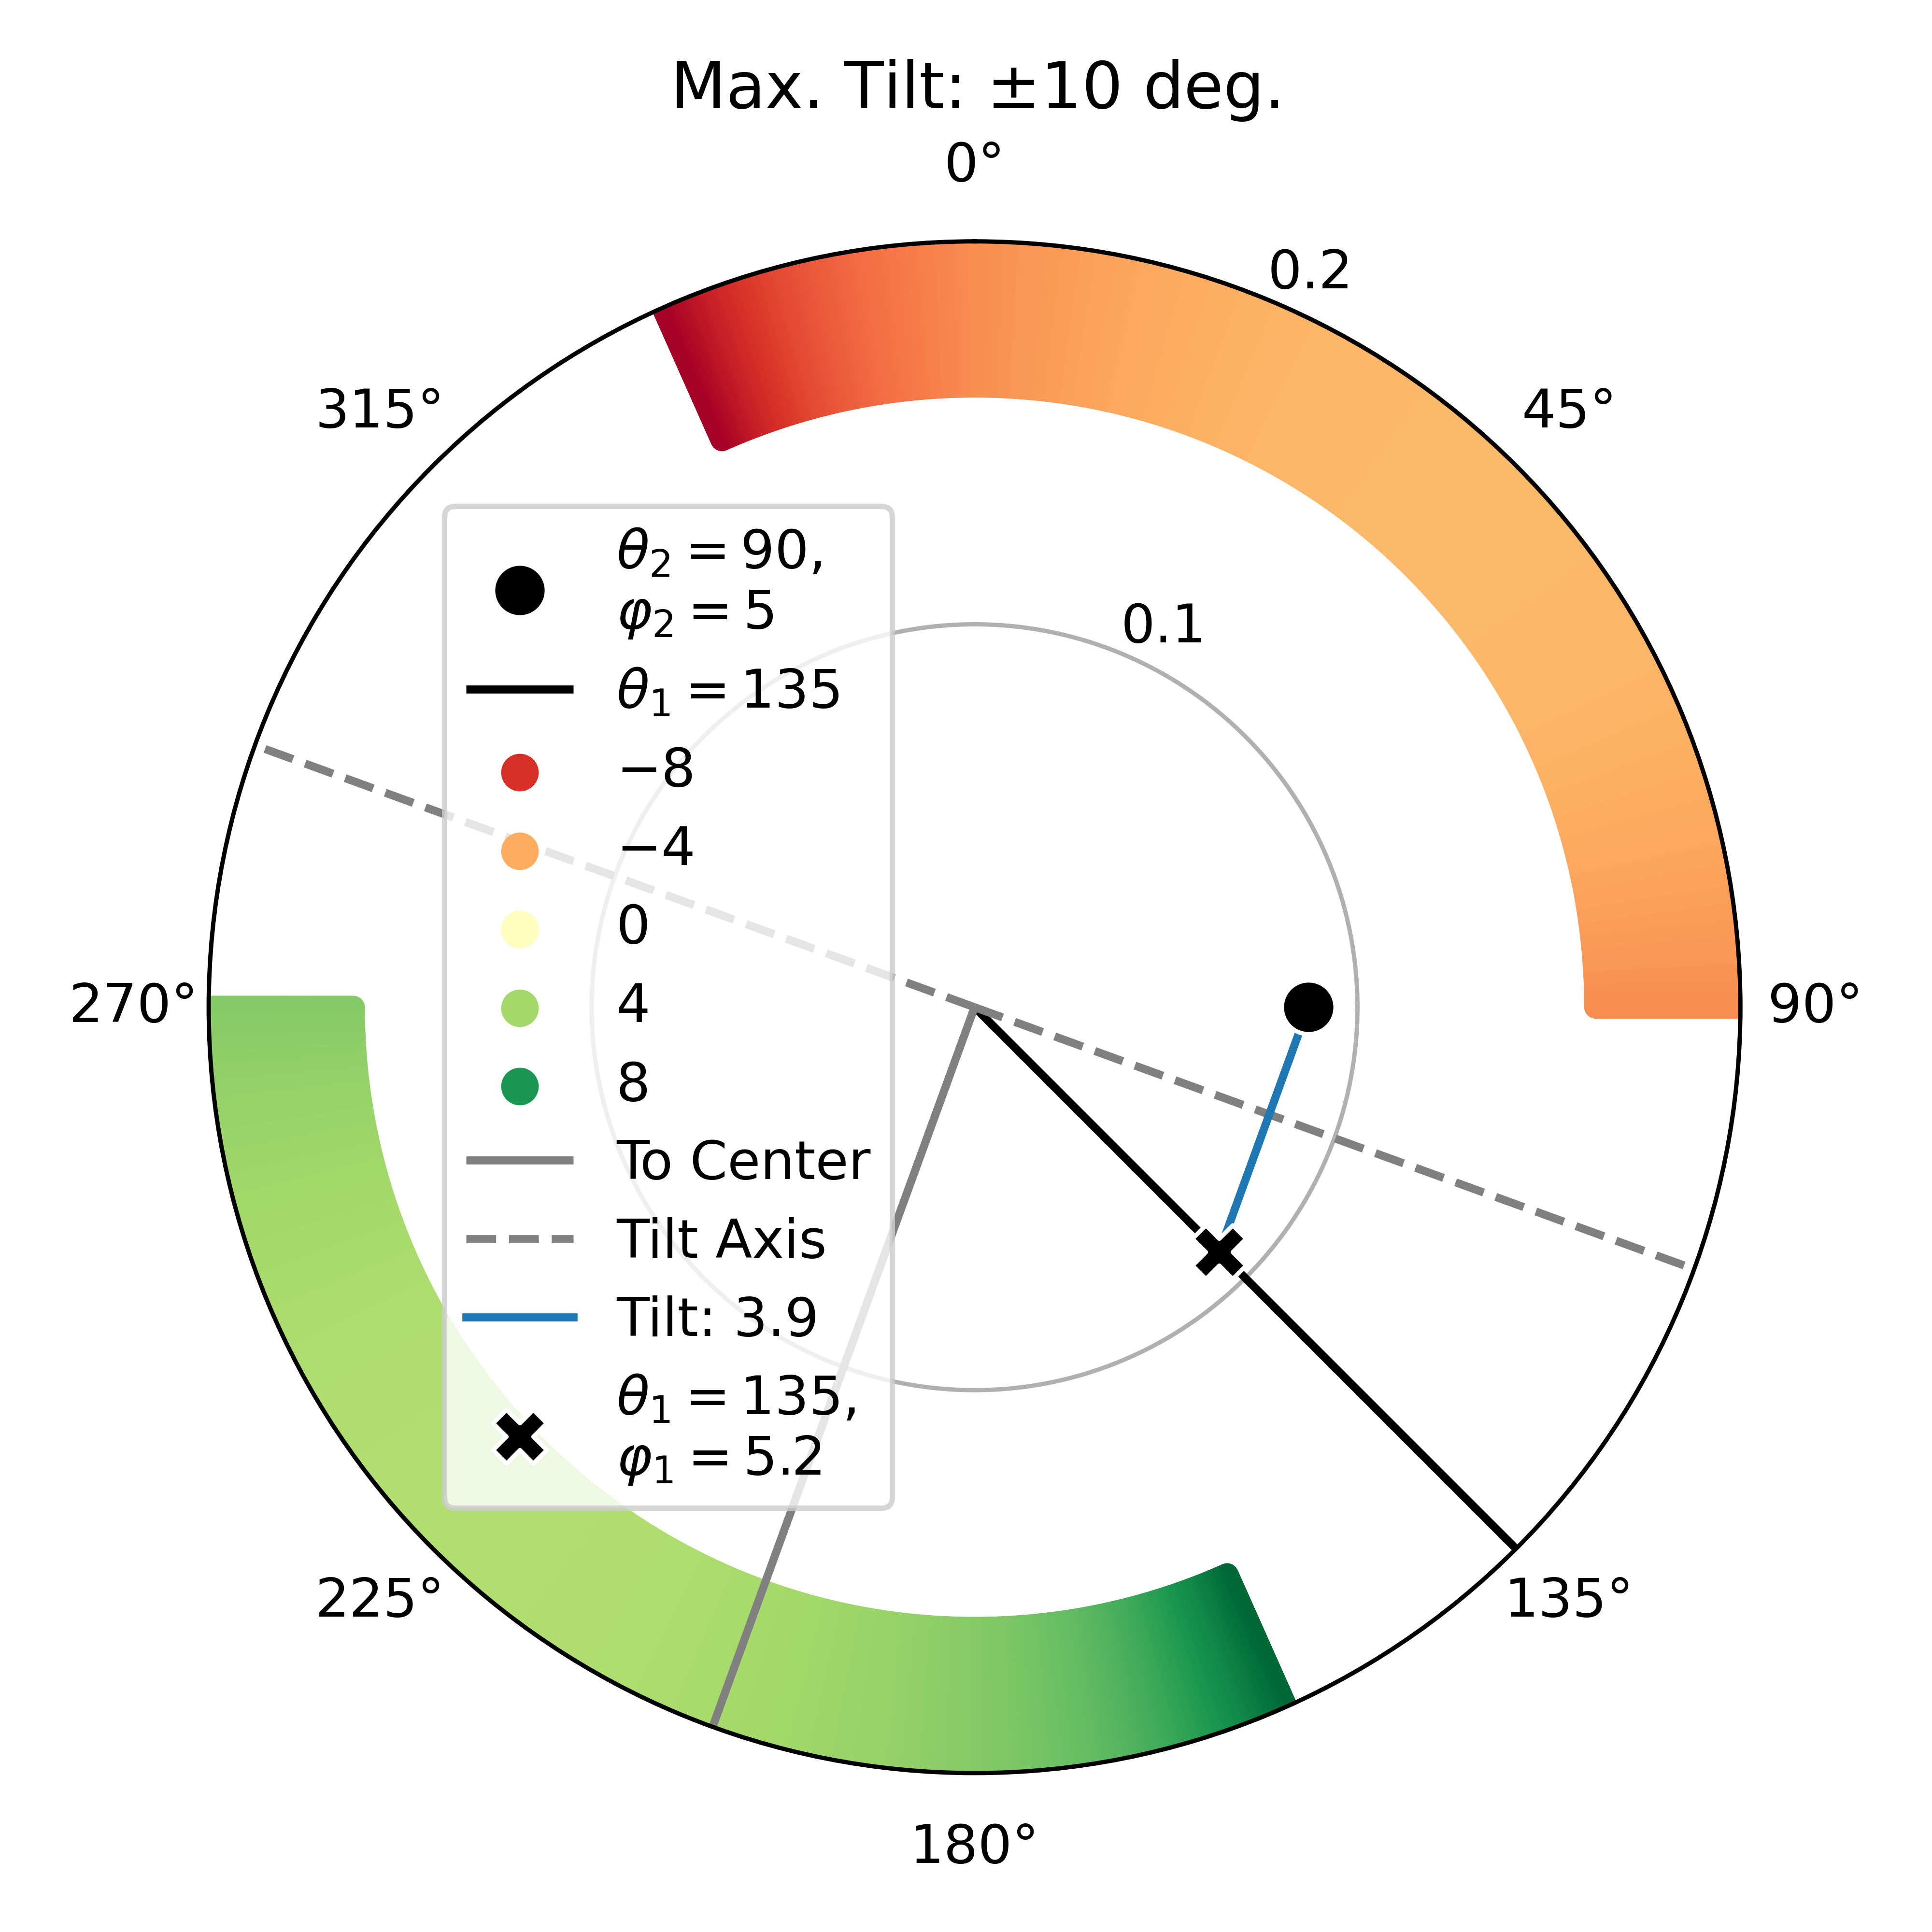
\includegraphics[width=.5\textwidth]{methods/tilt-check-example-rim.png}%
    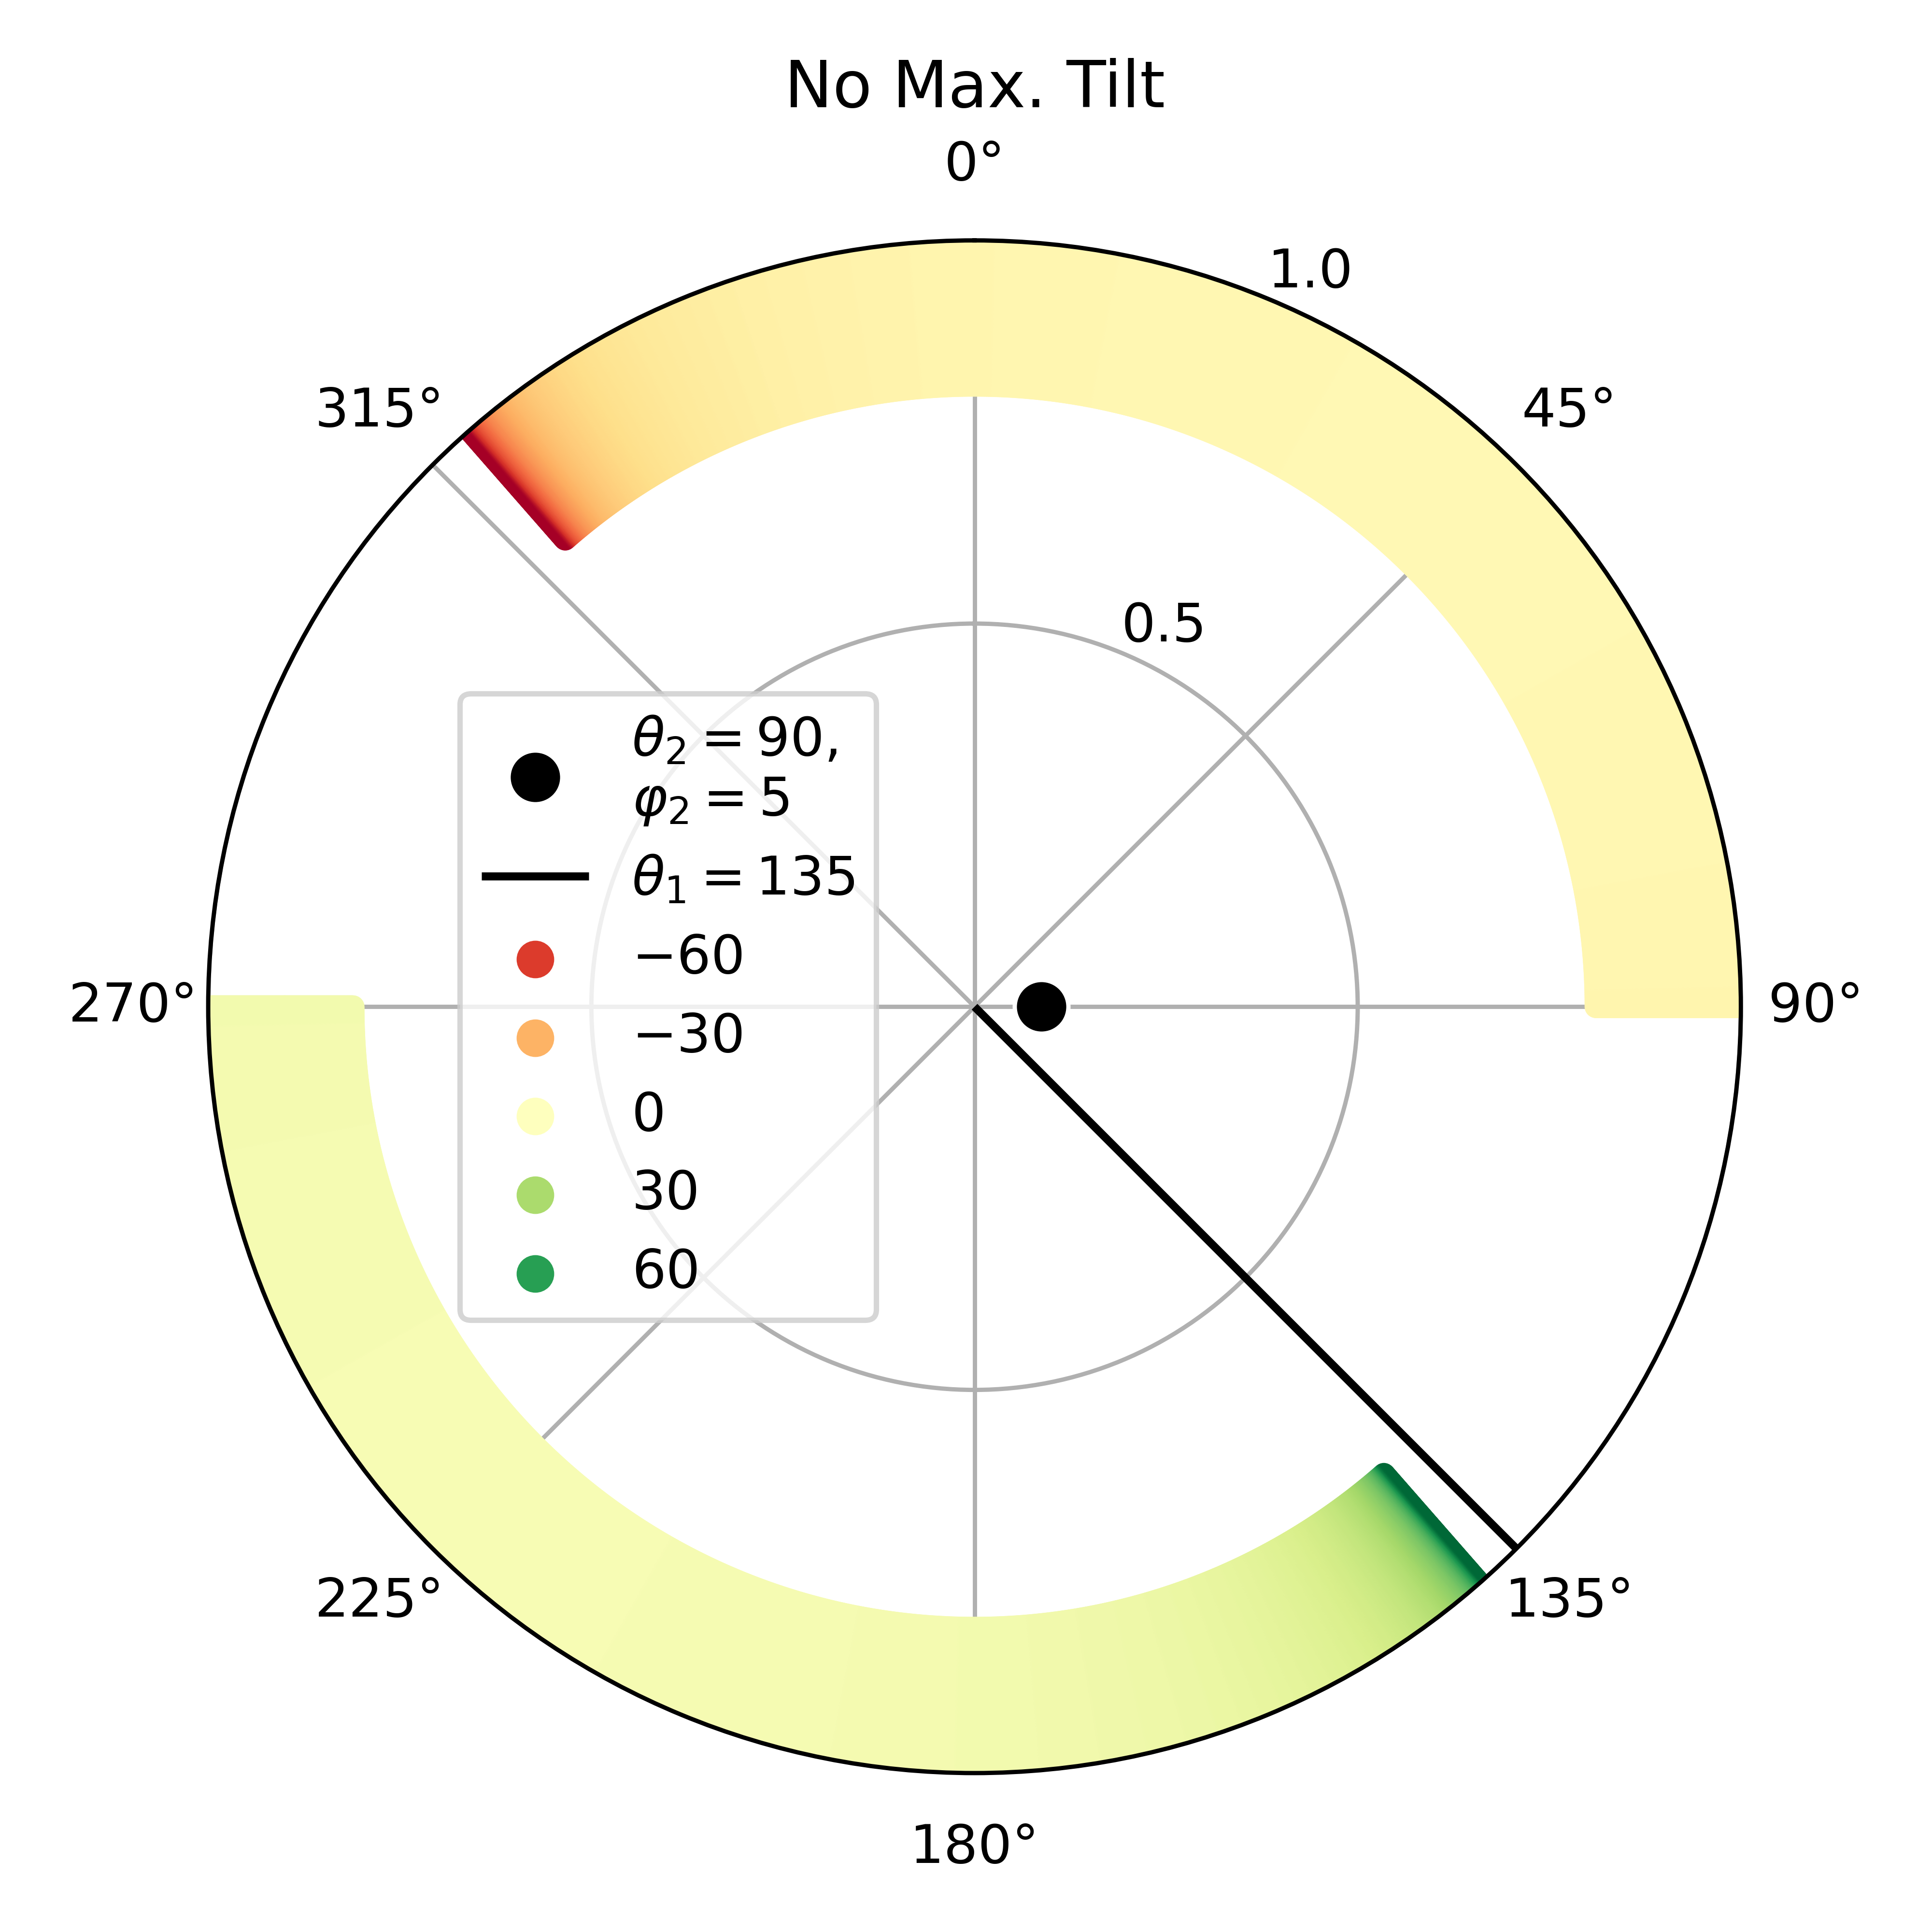
\includegraphics[width=.5\textwidth]{methods/tilt-check-rim.png}%
    \caption[Tilt calculation example]{Tilt calculation (Equation~\ref{eq:tilt-from-map}) example. \textbf{Top Left:} A discordant feature in an upper hemisphere orthographic projection, as in Figure~\ref{fig:attitude-data}. \textbf{Top Right:} A candidate inflation center to the SSW (North is \ang{0}) implies \ang{+3.9} degrees of tilt about the dashed tilt axis to sweep a paleo-attitude ($\times$) across the blue tilt-path to reach the modern attitude. Note the tilt path is perpendicular to the tilt axis and parallel to the center direction, as in Figure~\ref{fig:tilt-from-map}. \textbf{Bottom Left:} Tilt calculation repeated for all ``directions to center'' and assigned a color on the appropriate rim location. For example, the SSW center line intersects the light green color matching \ang{3.9} of tilt. Tilts exceeding \ang{10} excluded here to highlight variation. \textbf{Bottom Right:} Example removed for clarity. Tilts exceeding \ang{10} included. Note change in color ranges; all the centers shown in the lower left have the same values here.}
    \label{fig:tilt-example}
\end{figure}

\subsubsection{Offset Criterion}\label{sec:offset}

Section~\ref{sec:tiltable} introduces the ``tiltable'' criterion for samples with respect to a particular inflation center location. In particular, tilt estimates can only be obtained for certain values of the ``direction-away-from-center'' (\acs{bearing}) variable. The directions \emph{toward} these impossible centers are illustrated as the blank gaps in the colorful rims of Figure~\ref{fig:tilt-example} and described quantitatively in Section~\ref{sec:paleo-slope} (esp. Equation~\ref{eq:paleo-slope}).

However, it is also important to consider the reliability of these calculated tilt values. Notice in Figure~\ref{fig:tilt-example} that the highest-magnitude tilt calculations are densely clustered along one side of the \acs{bearing} line. The steep color gradient in this region indicates that tilt is sensitive to small variations in azimuth measurements of modern attitude, flow orientation, or center position. This unpredictable behavior approaches the undefined solution where the flow feature is colinear with the center candidate ($\acs{beta1}=\ang{0}$ or $\acs{beta1}=\pm\ang{180}$): no amount of tilt about the imposed axis can change the azimuth of the flow, so no tilt can be inferred from discordance (also illustrated in Figure~\ref{fig:discordance-concept}).

To avoid error-prone results captured by this phenomenon, I introduce an ``offset'' boolean criterion to complement the tiltable criterion. This criterion is simply a minimum cutoff value of \acs{beta1} of \ang{7}, chosen to capture most of the unstable behavior for typical attitude data in this thesis. More precisely, an ``offset'' sample relative to a particular center candidate is one where the absolute value of \acs{beta1} is greater than \ang{7} and less than $\ang{180} - \ang{7}=\ang{173}$. The tiltable and offset criteria are illustrated in Figure~\ref{fig:tiltable-offset}.

\begin{figure}
    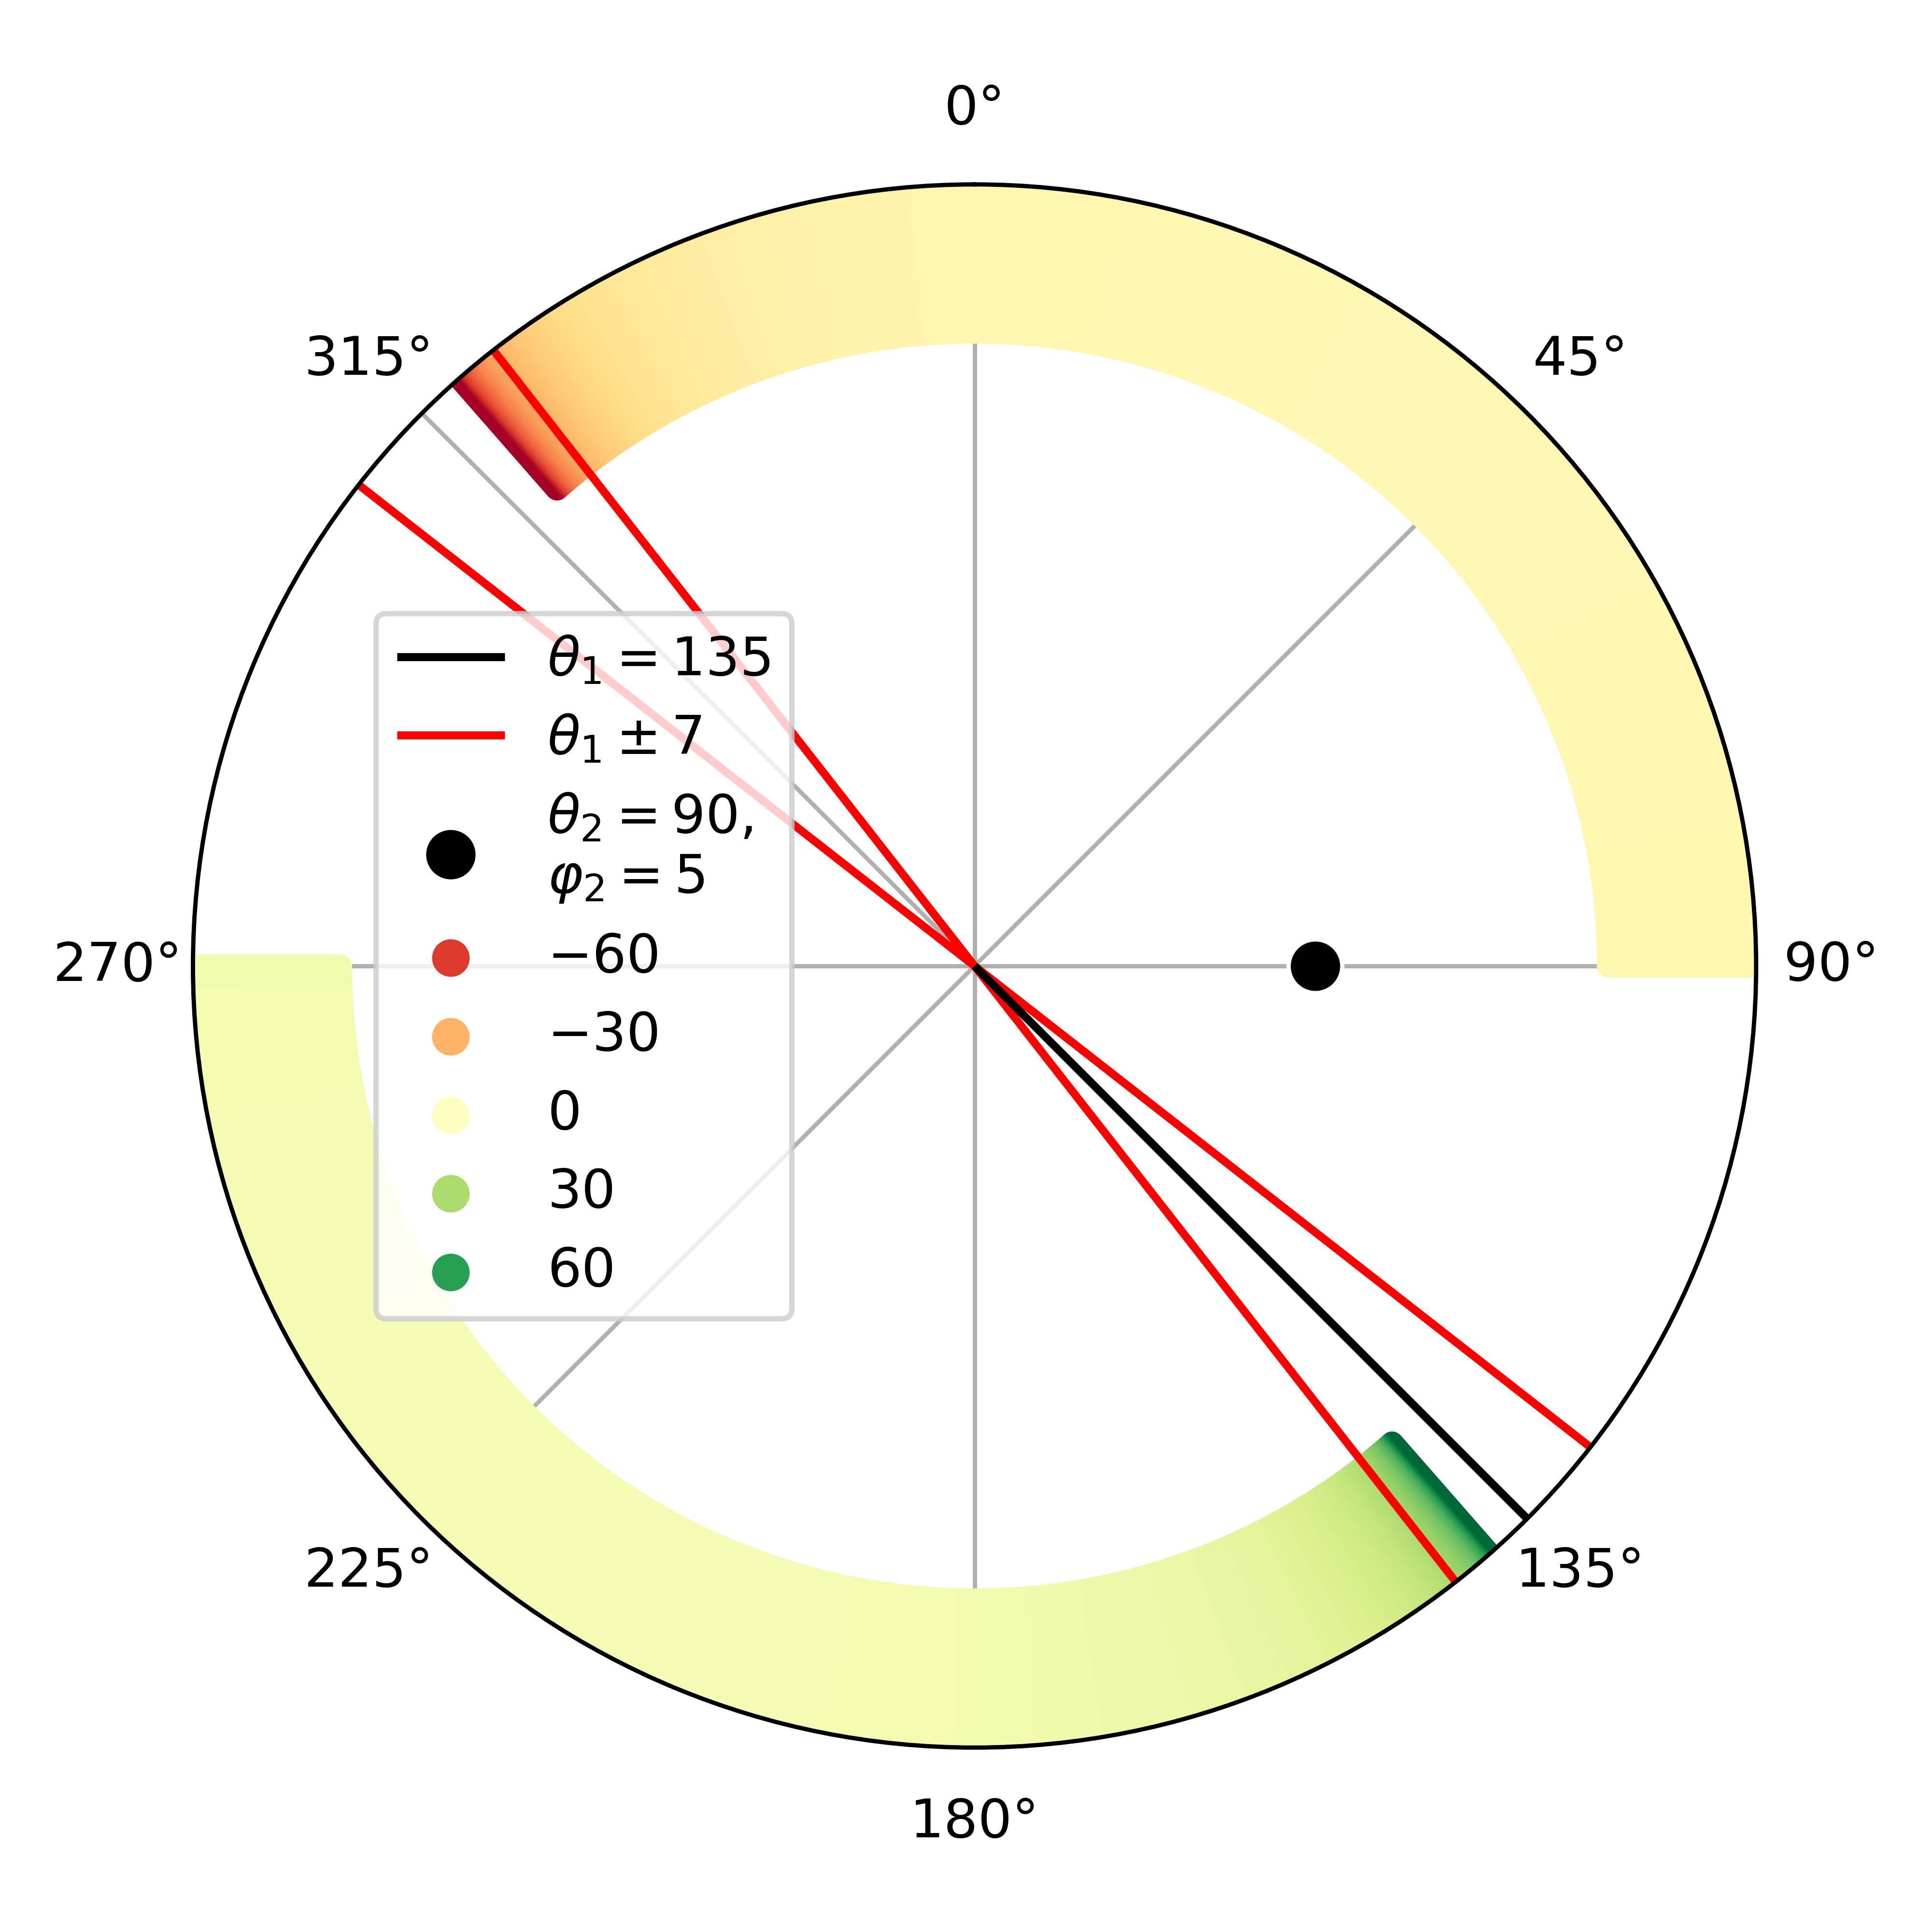
\includegraphics[width=\textwidth]{methods/tiltable-offset.png}%
    \caption[Sample criteria: tiltable/offset]{Two boolean criteria---tiltable and offset---used to assess how well a particular center describes a particular sample. For this sample, tiltable centers are those with a colorful rim (not the blank regions), where a tilt calculation can occur. Offset centers are those which are not within \ang{7} of colinear with the flow orientation; this region is bounded with red lines. Note that only direction-to-center matters for these criteria (not distance-to-center), since direction imposes the particular tilt axis (Figure~\ref{fig:tilt-example}). Note that a center-sample pair can be tiltable, offset, both, or neither, all of which are illustrated here.}
    \label{fig:tiltable-offset}
\end{figure}
\section{Assessing Reservoir Conditions}\label{sec:evaluation}

In this section I evaluate map-derived tilt-distance datasets generated in Section~\ref{sec:mapping} by comparison with model tilt-distance solutions from Section~\ref{sec:modeling}. The ultimate goal is to estimate an array of magma reservoir parameters---center position (map view), depth, radius (map view), aspect ratio, and pressure change---most consistent with the discordant flows at the surface. 

Among these five parameters of interest, reservoir center position must be assessed first because it alone dictates the tilt-distance dataset implied by a discordant set of features. This derived tilt-distance dataset can then be compared with an array of tilt-distance solutions derived from numerical models incorporating the other four parameters.

\subsection{Center Position}

Figure~\ref{fig:candidates} illustrates the array of candidates to be assessed as possible reservoir center locations. Section~\ref{sec:mapping} introduces the construction of a single tilt-distance data point from one discordant sample point relative to one center location. Repeating this calculation for all sample points relative to one center yields a full tilt-distance dataset corresponding to that center.\footnote{Figure~\ref{fig:tilt-example} illustrates instead repeating this calculation for a single sample point relative to all possible centers.} By repeating this construction, each center candidate can finally be evaluated on the basis of its associated tilt-distance dataset. In general, this means each dataset is reduced to a small set of numerical scores. This approach is outlined in Figure~\ref{fig:eval-model} and implemented in Appendix~\ref{app:code}.

\begin{figure}
    \begin{tikzpicture}[scale=.95]

  \usetikzlibrary{positioning}

\coordinate (ceval) at (0,0);
\coordinate (centersample) at (0,5);
\coordinate (samples) at (-3,10);
\coordinate (centers) at (3,10);

\node [rotate=270] at (7, 10) {Input (from GIS)};
\node [rotate=270] at (7, 5) {Intermediate list};
\node [rotate=270] at (7, 0) {Output (back to GIS)};

\draw[arrow,line width=1mm] (6, 10) -- (6, 0);

\node (samplestable) [draw, shape=rectangle, align=center] at (samples) {\begin{tabular}{c|c}
    sID & LAT, LON, \acs{az1}, \acs{az2}, \acs{sl2}\\
    \hline\\
    \hline\\
    \hline\\
    \hline\\
  \end{tabular}};

\node[above=0mm of samplestable] {\hltt{samples.csv}};

\node (centerstable) [draw, shape=rectangle, align=center] at (centers) {\begin{tabular}{c|c}
    cID & LAT, LON\\
    \hline\\
    \hline\\
    \hline\\
    \hline\\
    \hline\\
    \hline\\
  \end{tabular}};

\node[above=0mm of centerstable] {\hltt{centers.csv}};

\node (frontcentersample) [shape=rectangle, align=center, rounded corners=0.2cm] at (centersample) {\begin{tabular}{c|c|c}
  sID & LAT, LON, \acs{az1}, \acs{az2}, \acs{sl2} & \acs{dist}, \acs{bearing}, \acs{beta1}, \acs{beta2}, \acs{sl1}, \acs{tilt}\\
  \hline
  &\\
  &copy of & calculated\\
  &\hltt{samples.csv} & from one cID\\
  &\\
\end{tabular}};

\node[above=3mm of frontcentersample] {\hltt{centers\_calc}};

\foreach \x in {0.3,0.25,...,-0.05}
    \path (centersample) + (-\x, \x) node[draw, shape=rectangle, align=center, fill=white, rounded corners=0.2cm] {\begin{tabular}{c|c|c}
        sID & LAT, LON, \acs{az1}, \acs{az2}, \acs{sl2} & \acs{dist}, \acs{bearing}, \acs{beta1}, \acs{beta2}, \acs{sl1}, \acs{tilt}\\
        \hline
        &\\
        &copy of & calculated\\
        &\hltt{samples.csv} & from cID\\
        &\\
      \end{tabular}};

  \node (centersevaltable) [draw, shape=rectangle, align=center] at (ceval) {\begin{tabular}{c|c|c}
    cID & LAT, LON & SCORES\\
    \hline
    &\\
    &\\
    &copy of&each row calculated from\\
    &\hltt{centers.csv}&one item in \hltt{centers\_calc} \\
    &\\
    &\\
  \end{tabular}};

\node[above=0mm of centersevaltable] {\hltt{centers\_eval.csv}};

\end{tikzpicture}%
    \caption[Center evaluation workflow]{Schematic illustration of candidate center evaluation process. For each center (unique cID) in \hltt{centers.csv}, I make a copy of \hltt{samples.csv} and calculate variables for each sample (unique sID). This results in the ``intermediate list'' where each element corresponds to one cID. Then I evaluate each item in this list and write the resulting scores to one row of \hltt{centers\_eval.csv}.}%
    \label{fig:eval-model}
\end{figure}

Two broad questions inform the numerical scores assigned to each center based on its associated tilt-distance dataset:
\begin{enumerate}
    \item How well does the dataset capture the mapped discordant features?
    \item How well does the dataset capture a plausible modeled reservoir change event?
\end{enumerate}
Naturally, the best centers are the ones whose datasets can explain both the discordant features and a plausible reservoir change event. The following sections provide specific answers to these two questions. 

\subsubsection{Valid Fraction (Tiltable \& Offset)}\label{sec:valid-fraction}

Section~\ref{sec:tiltable} introduces the ``tiltable'' criterion for samples with respect to a particular inflation center location. In particular, tilt estimates can only be obtained for certain values of the ``direction-away-from-center'' (\acs{bearing}) variable. The directions \emph{toward} these impossible centers are illustrated as the blank gaps in the colorful rims of Figures~\ref{fig:tilt-example} and~\ref{fig:tilt-behavior} and described quantitatively in Section~\ref{sec:paleo-slope} (esp. Equation~\ref{eq:paleo-slope}).

However, even among the tiltable centers for a particular center,\footnote{Or, for this section, the tiltable \emph{samples} for a given \emph{center}.} it is also important to consider the reliability of the calculated tilt values. Notice in Figure~\ref{fig:fig:tilt-behavior} that the highest-magnitude tilt calculations are densely clustered along one side of the \acs{bearing} line. The steep color gradient in this region indicates that tilt is sensitive to small variation in azimuth measurements of modern attitude, flow orientation, or center position. This unpredictable behavior approaches the undefined solution where the flow feature is colinear with the center candidate ($\beta1=\ang{0}$ or $\beta1=\pm\ang{180}$): no amount of tilt about the imposed axis can change the azimuth of the flow, so no tilt can be inferred from discordance (also illustrated in Figure~\ref{fig:discordance-concept}).

To avoid error-prone results captured by this phenomenon, I introduce an ``offset'' boolean criterion to complement the tiltable criterion. This criterion is simply a minimum cutoff value of \acs{beta1} of \ang{7}, chosen to capture most of the unstable behavior for typical attitude data in this thesis. More precisely, an ``offset'' sample relative to a particular center candidate is one where the absolute value of \acs{beta1} is greater than \ang{7} and less than $\ang{180}-\ang{7}=\ang{173}$. The tiltable and offset criteria are illustrated in Figure~\ref{fig:tiltable-offset}.

\begin{figure}
    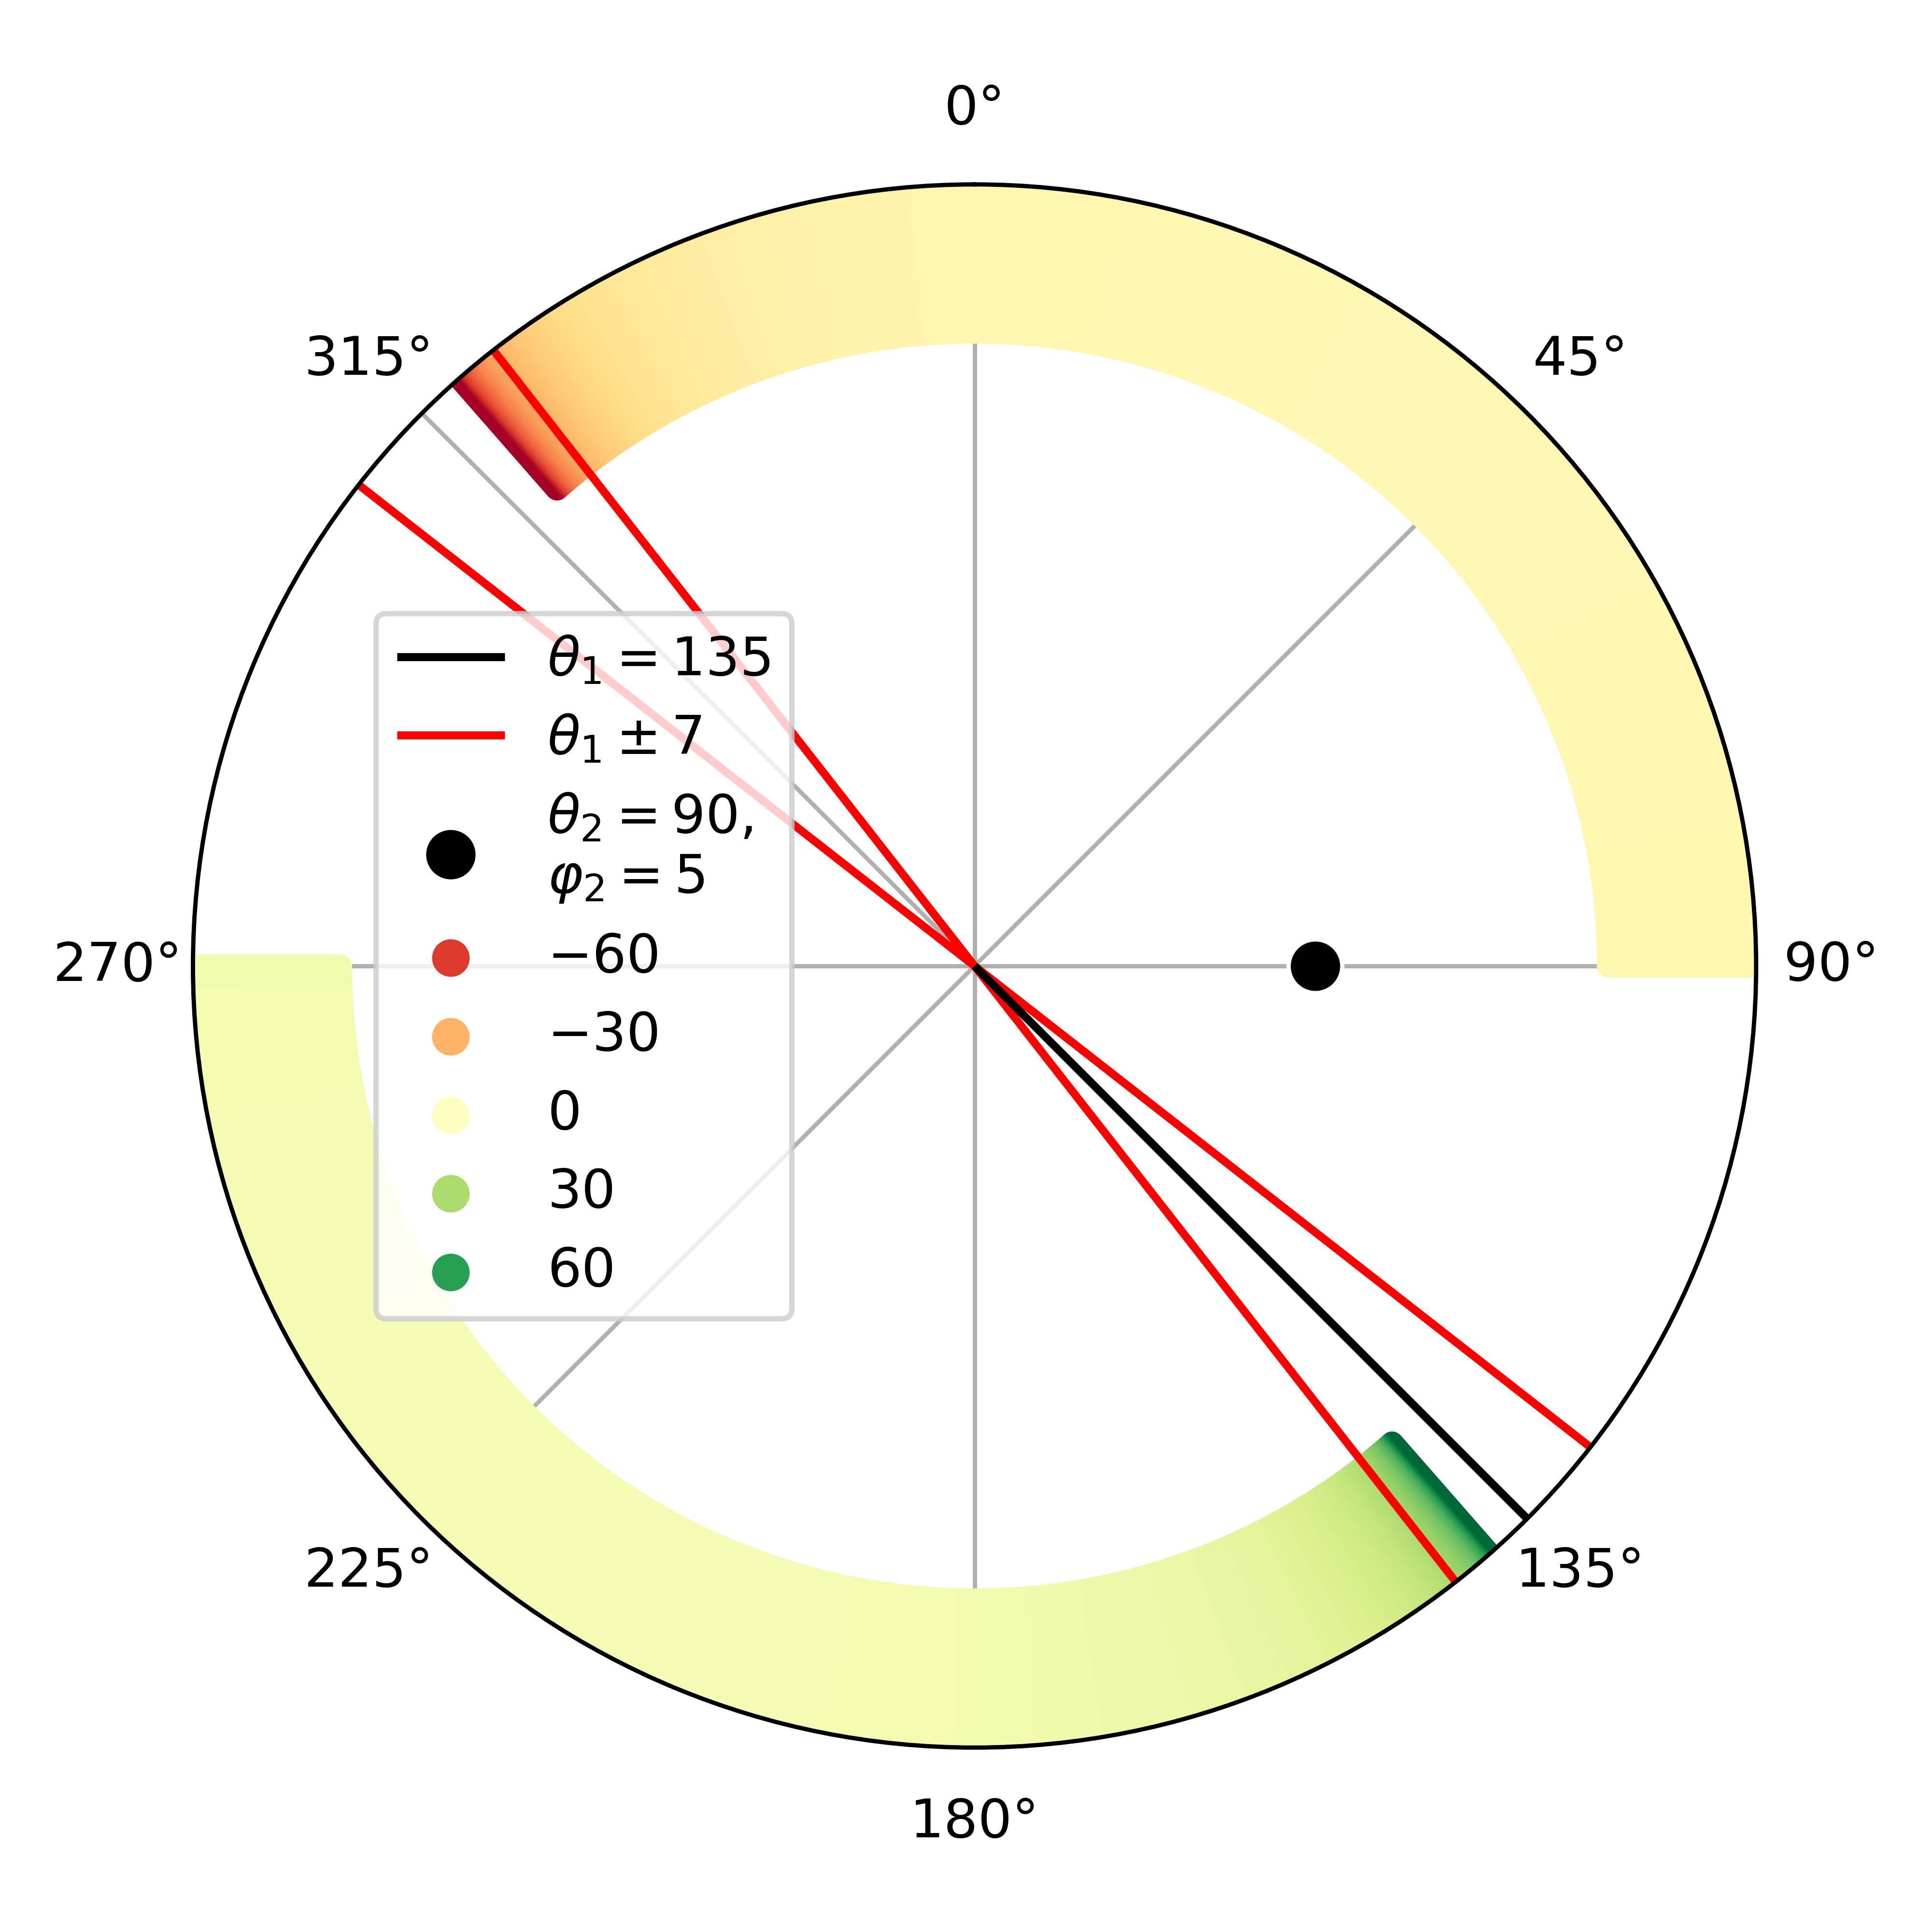
\includegraphics[width=\textwidth]{methods/tiltable-offset.pdf}%
    \caption[Sample Criteria: Tiltable \& Offset]{Two boolean criteria---tiltable and offset---used to assess how well a particular center describes a particular sample. For this sample, tiltable centers are those with a colorful rim (not the blank regions), where a tilt calculation can occur. Offset centers are those which are not within \ang{7} of colinear with the flow orientation; this region is bounded with red lines. Note that only direction-to-center matters for these criteria (not distance-to-center), since direction imposes the particular tilt axis (Figure~\ref{fig:fig:tilt-example}). Note that center-sample pair can be tiltable, offset, both, or neither, all of which are illustrated here.}
    \label{fig:tiltable-offset}
\end{figure}

A sample is well explained by a center if it is both tiltable and offset. Thus, an array of mapped samples is well explained by a center if a high fraction of those samples are both tiltable and offset. Thus, the score which captures how well each centers explains a particular set of discordant samples is the fraction of those samples which are both tiltable and offset.

\subsubsection{Goodness of Analytical Fit}\label{sec:inflation-center}

Instead, I need to consider a larger population of tilt-distance data points together. This increases the likelihood of recognizing a tilt pattern consistent with reservoir pressure change, i.e., a shape similar to those shown in Figures~\ref{fig:grav-topo-test},~\ref{fig:mogi-test}, and~\ref{fig:mogi-test-shallow-oblate}.

Finally, I perform a least-squares regression\footnote{Implemented using the \hltt{curve\_fit} function from the \hltt{scipy.optimize} Python module \parencite{2020SciPy-NMeth}} to fit an analytical tilt solution (Equation~\ref{eq:mogi-tilt}) to the valid sample subset (tiltable \& offset). Just as a linear regression computes the best-fitting slope and intercept, this process computes the best-fitting depth and energy parameters. In both cases, the best fit minimizes the mean square error:
\begin{equation}
    \frac{1}{n}\sum_{i}^{n}{\left[\acs{tilt}_i-\hat{\acs{tilt}}_i\right]}^2\label{eq:mse}
\end{equation}
for $n$ observations of the form $(\acs{dist}, \acs{tilt})$ where $\hat{\acs{tilt}}$ is evaluated at $\acs{dist}$ using the best-fit parameters. The details of the curve-fitting algorithm (Levenberg-Marquardt) are beyond the scope of this thesis, but one important difference from a simpler linear regression model is that the curve does not necessarily converge (successfully estimate a set of best-fitting parameters) for particularly messy datasets. Whether convergence occurs (and even the final parameter estimates) depends on initial parameter estimates and maximum number of iterations allowed before ``giving up'' on convergence.

Initial parameter estimates for inflation energy $\acs{epv} = \qty{7e19}{\J}$ if the mean tilt in the dataset is positive and \qty{-7e19}{\J} if the mean is negative. The initial depth estimate is $d = \qty{20}{\km}$ in either case. 500 iterations are allowed before a dataset is deemed non-convergent, i.e., not explainable by an analytical tilt model in the form of Equation~\eqref{eq:mogi-tilt}.

After performing each regression, I first assess the mathematical goodness of fit for each center's fitted tilt solution. First, I determine what fraction of the samples are. Recall that the regression only proceeds using this subset, so the fraction of the dataset involved provides important context for the second criterion: what is the \ac{RMSE} of the regression, if one converges at all? This statistic is the square root of Equation~\eqref{eq:mse}:
\begin{equation}
    \sqrt{\frac{1}{n}\sum_{i}^{n}{\left[\acs{tilt}_i-\hat{\acs{tilt}}_i\right]}^2}.\label{eq:rmse}
\end{equation}
It has the same units as \acs{tilt} (degrees) and provides a relative comparison of goodness-of-fit for regression results; smaller values indicate better fit. Taken together, the tiltable fraction and \ac{RMSE} associated with each center reflect the mathematical goodness-of-fit for each center candidate.

I use these fitted values and crucially, their associated error terms, to determine the likelihood that surface tilt actually occurred in the direction radial to the given center candidate. This approach is supported by Figure~\ref{fig:mogi-test-shallow-oblate}, which illustrates that even tilt resulting from shallow, oblate reservoirs within a topographic edifice can be fit well to the analytical Mogi tilt function. At this stage, I pay closer attention to the parameter error estimates (similar to an $R^2$ value for a linear regression) to determine whether \emph{any} axisymmetric tilt is likely to have occurred from this center, rather than the estimates themselves---although I treat any unrealistic parameter estimates with caution regardless of their goodness of fit.

This sequence of calculations is much more computationally expensive than the previous one, and a single realistic reservoir pressure change is unlikely to explain the entire dataset anyway. Therefore, I select smaller sample populations for this criterion, paying particular attention to the highly discordant flows near the southern summit region shown in Figure~\ref{fig:uphill-flows}.

\subsection{Depth, Radius, Aspect Ratio, \& Pressure Change}

After narrowing down the set of plausible inflation center locations (map view) in Section~\ref{sec:evaluation}, I use numerical model results to refine estimates for reservoir size, depth, shape, and pressure change.

Section~\ref{sec:evaluation} narrows down the plausible horizontal position of the reservoir center, but it can only play a limited role in identifying volcanologically plausible configurations.

Figure~\ref{fig:mogi-test-shallow-oblate} illustrates a key preliminary finding: map data which are well explained by an analytical Mogi tilt solutions are also likely to fit one or numerical results which approximate the deep, point-like reservoir assumed by \textcite{mogi_relations_1958}. Disagreement between numerical and analytical increases with the degree of analytical assumption violations.

The magmatic system below the summit of Olympus Mons is likely shallow and oblate. 

I use the same iterative optimization method (minimizing \acs{RMSE}) described in Section~\ref{sec:inflation-center}. In the absence of an explicit tilt equation parameterized by reservoir size, depth, shape, and pressure change, I perform a brute-force search through an array of numerical solutions at each iteration.

For each dataset (corresponding to a center candidate of interest) this process begins with a very coarse set of numerical model parameters. I use the \hlss{Parametric Sweep} tool in COMSOL to define a list of values to test for each parameter; the software produces and exports a displacement solution for each one. After
\chapter{Results}\label{cha:results}

\section{Mapping Coverage}

Figure~\ref{fig:features} depicts mapped polygonal flows and linear channels; Figure~\ref{fig:samples} shows the samples derived from these features symbolized by discordance (\acs{disc}). Polygonal appear throughout the study area but are concentrated immediately to the west and southeast of the caldera complex. Linear flow channels are distributed more evenly around the study area, particularly in the southern half. Figure~\ref{fig:samples} shows the spatial distribution of sampled points by discordance; Figure~\ref{fig:discordance} illustrates the statistical distribution of computed discordance values. 

\begin{figure}
    \includegraphics[width=\textwidth]{results/features.pdf}%
    \caption[Mapped lava features]{Mapped polygonal lava flows and linear channels. Note the greater density of identifiable flows to the west and southeast of the caldera complex, with channels distributed more evenly around the study area---especially in the southern half.}%
    \label{fig:features}
\end{figure}

\begin{figure}
    \includegraphics[width=\textwidth]{results/samples.pdf}%
    \caption[Spatial distribution of discordance]{Samples symbolized by topographic discordance. Note that the most discordant ($|\acs{disc}|\approx\ang{180}$) samples are tightly clustered around the caldera rim. Only the southeast region (part of which is shown in Figure~\ref{fig:uphill-flows}) shows nearly reversed flows beyond \qty{\sim10}{\km} from the complex.}%
    \label{fig:samples}
\end{figure}

\begin{figure}
    \includegraphics[width=\textwidth]{results/discordance.pdf}%
    \caption[Statistical distribution of discordance]{Most of the 565 sampled points correspond to lava features whose azimuths diverge from the topographic downhill direction by a few tens of degrees.}%
    \label{fig:discordance}
\end{figure}

The goal of this thesis is to assess elastic deformation recorded in discordant lava features. Just as important as identifying suitable regions of discordance for analysis is removing regions for which the inherent attitude data incompleteness inhibits analysis. To see this, consider Figure~\ref{fig:full-tiltable-offset}, which illustrates the paradox of the discordance method. After all the discussion of axisymmetric geometry in this thesis, one might expect the center of the (roughly) axisymmetric volcanic edifice to play a central role in assessing subsurface reservoir pressure change. Instead, this is precisely the region where the discordance method is least robust, since most of the flow and channel samples are not offset enough that pressure change would produce significant or predictable discordance. Instead, it is only the \emph{asymmetry} of the magmatic system that can be assessed here. 

\begin{figure}
    \includegraphics[width=\textwidth]{results/full-tiltable-offset.pdf}%
    \caption[Tiltable/Offset Fraction (Full Dataset) REPLACE]{REPLACE. The lava features in the study area are largely radial to the caldera center, as expected in a shield volcano. The caldera center is also the most plausible pressure change center; however, this is precisely the region which cannot be explained using the discordance method because resulting inflation does not cause lava features to change their downhill azimuth. Note here that the candidates within the caldera are the least plausible because very few of the samples in the full dataset are offset with respect to those centers.}
    \label{fig:full-tiltable-offset}
\end{figure}

To assess asymmetric elements of the magmatic system, I reduce the sample dataset to the subset whose discordance signature is most likely to record elastic deformation. Figure~\ref{fig:populations} shows three sample populations selected within a highly discordant region for inflation center evaluation.

\begin{figure}
    \includegraphics[width=\textwidth]{results/populations.pdf}%
    \caption[Sample populations for inflation center evaluation]{I use three nearby populations of lava features from which to evaluate axisymmetric inflation candidates. These are among the most discordant features in the summit which are not immediately adjacent to the immediate caldera rim. For reference, the flows shown in the center of Figure~\ref{fig:uphill-flows} are included in population B.}%
    \label{fig:populations}
\end{figure}

These three populations are analyzed together but labeled separately to orient the reader and confirm distance calculations behave as expected. For example, a tilt-distance dataset corresponding to a center in the southern summit region should have C as the closest and A as the furthest.

Figure~\ref{fig:tiltable-offset-abc} illustrates the tiltable/offset fraction of these populations relative to the array of center candidates. As expected, the NW-SE trending non-offset region (colinear with most of the features) contains the least plausible inflation center candidates---those with the lowest tiltable/offset fraction. However, the northeast side of this region is notably more plausible than the southwest side.

\begin{figure}
    \includegraphics[width=\textwidth]{results/tiltable-offset-abc.pdf}%
    \caption[Centers by tiltable/offset fraction]{Centers which yield a well-constrained (offset) quantitative tilt estimate (tiltable) for the highest proportion of the discordant features in the southeast summit. Note the red streak roughly colinear with the lava features: centers in this region are not offset, i.e., tilt about the imposed axis tends to change slope but not downhill azimuth. Note also the asymmetry across this central red streak; centers north of the samples (near the eastern caldera rim) are more plausible than those to the west (southern summit, near Pangboche crater). Additional regions of high tiltable/offset fraction occur directly within the populations and in the far northwest corner of the caldera complex.}%
    \label{fig:tiltable-offset-abc}
\end{figure}


Figure~\ref{fig:rmse-abc} illustrates the analytical least-squares regression results for the tiltable/offset fraction of each center's tilt-distance dataset. These results are consistent with, and provide additional context for, Figure~\ref{fig:tiltable-offset-abc}. In particular, much of the non-offset central red region either does not converge or converges to a physically meaningless result.\footnote{Specifically, regression results are excluded for two cases depending on the maximum estimated tilt. If the maximum (or most negative) tilt is within \ang{0.1}, the center is excluded as recording essentially no deformation. On the other hand, a few analytical regression results converge with a physically impossible tilt of \ang{180}, again failing to capture physical deformation.} The main exception to this trend is a few centers which converge poorly ($\acs{RMSE}\approx\ang{10}$) just at the southern rim of the largest caldera floor. Additionally, the only convergent centers in the southeast division occur near the modern summit east of Pangboche crater. These converge to positive \acs{epv} (inflation), while the rest of the centers converge to negative \acs{epv} (deflation).

Nearly all the centers in the northeast division (within/outside the eastern caldera complex) converge. Note that while these centers have slightly higher \acs{RMSE} values than those in the southern summit region, they are not necessarily ``better'' fits because the tiltable/offset fraction (sample size for regression) is significantly less in the southern summit than it is in the eastern caldera rim.

\begin{figure}
    % flatten pdf annotations: https://tools.pdf24.org/en/flatten-pdf#s=1681704380798
    \includegraphics[width=\textwidth]{results/rmse-abc.pdf}%
    \caption[Centers by analytical convergence]{Centers for which an analytical tilt solution converges on the tiltable/offset subset (Figure~\ref{fig:tiltable-offset-abc}) of the southeast populations. Blank regions either do not converge at all or converge to a physically meaningless solution. Note that both inflation from the south (black circles) or deflation from the north (plain circles) are consistent with the same regional tilt pattern back toward the eastern caldera complex. Key regions numbered for further inspection of associated tilt-distance datasets. Regions 1-5 are promising with relatively low \acs{RMSE} and high tiltable/offset fraction; 6 \& 7 illustrate important limitations of the method.}%
    \label{fig:rmse-abc}
\end{figure}

Figures contain specific representative tilt-distance datasets for centers within each of four regions of interest labeled in Figure~\ref{fig:rmse-abc}:

\begin{enumerate}
    \item Southeast caldera rim (Figure~\ref{fig:region1-analytical})
    \item East of caldera rim (Figure~\ref{fig:region2-analytical})
    \item Southern summit (Figure~\ref{fig:region34-analytical})
    \item Within discordant features (Figure~\ref{fig:region34-analytical})
\end{enumerate}

\begin{figure}
    \vspace{-15pt}
    \includegraphics[width=\textwidth]{results/428-analytical.pdf}\\
    \includegraphics[width=\textwidth]{results/486-analytical.pdf}\\
    \includegraphics[width=\textwidth]{results/544-analytical.pdf}%
    \caption[Southeast Caldera Rim: analytical fit]{Representative datasets for centers in region 1 (southeast caldera rim). Vertical tick marks represent distances to all samples. Scatter points represent tilt computed for the tiltable/offset samples. The analytical fit for each dataset is labeled with its \acs{RMSE}, \ang{\sim2.7} for the best fits. Despite high error, note the tilt signature is consistently negative, i.e., represents deflation as expected.}
    \label{fig:region1-analytical}
\end{figure}

\begin{figure}
    \vspace{-15pt}
    \includegraphics[width=\textwidth]{results/403-analytical.pdf}\\
    \includegraphics[width=\textwidth]{results/432-analytical.pdf}\\
    \includegraphics[width=\textwidth]{results/549-analytical.pdf}%
    \caption[East of Caldera Rim: analytical fit]{Representative datasets for centers in region 2 (east of caldera rim).}
    \label{fig:region2-analytical}
\end{figure}

\begin{figure}
    \includegraphics[width=\textwidth]{results/17-analytical.pdf}\\
    \includegraphics[width=\textwidth]{results/24-analytical.pdf}\\
    \includegraphics[width=\textwidth]{results/151-analytical.pdf}%
    \caption[East of Caldera Rim: analytical fit]{Representative datasets for centers in region 3 (southern summit).}
    \label{fig:region34-analytical}
\end{figure}

\section{Depth, Radius, Aspect Ratio, \& Pressure Change}

\begin{figure}
    \includegraphics[width=\textwidth]{results/486-numerical-fits.pdf}\\
    \includegraphics[width=\textwidth]{results/486-cross-sections.pdf}%
    \caption[486 Numerical Fits]{Numerical fits for center 486 (Region 1; southeast caldera rim). Several reservoir configurations fit the dataset better than the analytical solution. Note that numerical tilt solutions can improve this fit in multiple ways; the shallow tilt solution is qualitatively different from the medium and deep solutions. Note that the two deeper reservoirs of similar shape yield similar solutions by balancing depth with pressure change magnitude. Meanwhile, a smaller shallow reservoir yields a numerical tilt solution which improves the analytical fit in a different direction.}
    \label{fig:486-numerical-fits}
\end{figure}
\chapter{Discussion}\label{cha:discussion}

The central goal of this thesis is to determine the extent to which discordant features at the summit of Olympus Mons can provide insight into the magma system below the surface. Researchers have approached this problem at a larger scale 

Under the assumption that lava flows record the downhill direction at the time of their emplacement, discordant lava features have long been used to infer surface deformation responsible for this discrepancy. This method has been applied at a regional scale to constrain flexural loading of the lithosphere from large volcanic edifices \parencite{mouginis-mark_ancient_1982,isherwood_volcanic_2013,chadwick_late_2015} and more recently to reservoir-scale processes at the summit of Olympus Mons \parencite{mouginis-mark_late-stage_2019}. In this thesis, I use topographic discordance as a starting point but acknowledge the fundamental limitation that downhill azimuth of a lava feature is insufficient for fully describing the attitude of the surface upon which it was emplaced. A full description of paleo-attitude is crucial because it can be directly compared with the modern attitude to determine the degree of deformation that has taken place at the location of a discordant feature. Thus the overarching problem I set out to solve in Chapter~\ref{cha:methods} is completing this dataset in a physically plausible and volcanologically useful way. After solving this problem, I can compare the tilt between mapped paleo- and modern attitudes to the tilt resulting from modeled reservoir pressure change at depth.

\section{Limitations}

Only a fraction of the study area surface is covered in flows whose orientation can be reliably determined. These flows are of different ages. They record an incomplete picture of the topographic surface upon which they were emplaced. Only those which were subsequently deformed off-axis (i.e., by an offset center, or a more complex inflation system with the same net tilt axis) become discordant. In this case, the majority of pressure change appears to have been minimally offset, if at all.

\section{Future Directions}

\subsection{Crater Counting}
Important progress has been made toward constraining the timeline of Late Amazonian volcanic activity using crater counting \parencite{kneissl_map-projection-independent_2011,robbins_volcanic_2011,
robbins_large_2013,
platz_crater-based_2013}, although a detailed chronology is still out of reach. The difficulty inherent to the stochastic nature of this method is that small regions are difficult to date with high precision. One result from this thesis which could address this challenge is that discordant populations which are best explained by the same axisymmetric pressure change conditions are likely to have been deformed (if not emplaced) at the same time. Conversely, populations whose most likely centers differ in position and inflation energy are more likely to be stratigraphically distinct. While the method of this thesis cannot directly resolve relative ages, it could help to identify contemporaneous units and thus increase the precision of the crater counting method by expanding the area of interest.

\subsection{Morphological Constraints on Paleo-slope}

The fundamentally missing piece of attitude data (which the whole axisymmetric tilt framework is designed to estimate) is paleo-slope: the slope of the surface upon which a lava feature was originally emplaced. The paleo-slope values that I calculate could be compared with independent constraints on paleo-slope based on the morphology of lava flows \parencite{wadge_lobes_1991, peitersen_correlations_2000, peters_lava_2021} to assess plausibility of the axisymmetric assumption I use to derive these estimates.

\subsection{Evaluating Model Conditions}

Finally, it will be important to bring the tilt analysis beyond analytical regression fit to more careful consideration of a range of reservoir parameters. After making these more specific estimates, numerical modeling can provide more sophisticated criteria for physical plausibility than the simple cutoff envelope used here. For example, it will be important to determine whether estimated parameters would cause reservoir wall failure before the estimated pressure needed to explain the tilt signature would physically be able to accumulate. 
\chapter{Conclusions}

In this thesis I develop a geometric framework for estimating the location and inflation energy of magma reservoir pressure to explain surface deformation implied by topographically discordant lava features. I focus on justifying this method of mathematical and physical grounds, paying particular attention to the impact of simplifying assumptions applied throughout the process. Preliminary results from this method are intended as an early but promising proof-of-concept, with significant challenges still requiring careful attention before volcanological insight can be derived with confidence.

%\chapter*{Acknowledgements}
\addcontentsline{toc}{chapter}{Acknowledgements}

I would first like to thank my thesis advisor Dr.\ Eric Grosfils for his insightful guidance on this project and throughout my time at Pomona College.

I would also like to thank my academic advisor Dr.\ Masha Prokopenko.

Finally, I have to thank the thousands of documentation authors, StackOverflow contributors, YouTube tutorial creators, blog writers, and other online educators who have all unknowingly made this work possible. 

\begin{flushleft}
    \printbibliography[heading=bibintoc]
\end{flushleft}

\appendix % lettering
\chapter{Spherical Trigonometry}\label{app:spherical-trig}
Let two poles be defined in attitude space $(\theta,\varphi,\rho)$ on the unit sphere $(\rho=1)$ by:
\begin{equation}
    p=(\theta_p,\varphi_p,1)\qquad q=(\theta_q,\varphi_q,1).
\end{equation}
Let a cartesian coordinate system $(x,y,z)$ be defined such that $\hat x$ is parallel to $\theta_p$, $\hat y$ is \ang{90} counter-clockwise from $\hat x$, and $\hat z$ is parallel to the spherical zenith. Then, $p$ and $q$ take the following form: % as shown in Figure~\ref{fig:spherical-cosines}
\begin{equation}
    p=
    \begin{bmatrix}
        \sin\varphi_p\\
        0\\
        \cos\varphi_p
    \end{bmatrix}
    \qquad
    q=
    \begin{bmatrix}
        \sin\varphi_q\cos\beta\\
        \sin\varphi_q\sin\beta\\
        \cos\varphi_q
    \end{bmatrix},
\end{equation}
where $\beta=\theta_q-\theta_p$. I use the dot product compute the central angle $\alpha$ subtended by $p$ and $q$:
\begin{equation}
    p\cdot q
    =\|p\|\,\|q\|\cos\alpha
    =p_{x}q_{x}
    +p_{y}q_{y}
    +p_{z}q_{z}.\label{eq:dot-product}
\end{equation}
Since $\|p\|=\|q\|=1$ by construction, Equation~\eqref{eq:dot-product} reduces to:
\begin{gather}
    \cos\alpha
    =\sin\varphi_p\sin\varphi_q\cos\beta
    +\cos\varphi_p\cos\varphi_q,\nonumber\\
    \alpha
    =\arccos(\sin\varphi_p\sin\varphi_q\cos\beta
    +\cos\varphi_p\cos\varphi_q).
\end{gather}

% \begin{figure}
%     \begin{center}
%         \input{figures/spherical-cosines.tex}%
%         \caption[Spherical law of cosines]{Geometric view of spherical law of cosines}%
%         \label{fig:spherical-cosines}%
%     \end{center}
% \end{figure}

For constant $\beta$ and $\varphi_q$, the value of $\varphi_p$ which minimizes $\alpha$ (great circle distance) can be calculated by setting:
\begin{equation}
    \frac{\partial}{\partial \varphi_p}
    \arccos\left(\sin\varphi_p\sin\varphi_q\cos\beta
    +\cos\varphi_p\cos\varphi_q\right)
    =0.\label{eq:mimimum}
\end{equation}
Differentiating using the chain rule,
\begin{equation}
    \frac{-\,(\cos\varphi_p\sin\varphi_q
    \cos\beta-\sin\varphi_p\cos\varphi_q)}
    {\sqrt{1-{(\sin\varphi_p\sin\varphi_q\cos\beta
    +\cos\varphi_p\cos\varphi_q)}^2}}
    =0.\label{eq:derivative}
\end{equation}
Multiplying through by the denominator and rearranging to solve for $\varphi_p$:
\begin{gather}
    \cos\varphi_p\sin\varphi_q
    \cos\beta-\sin\varphi_p\cos\varphi_q
    =0,\nonumber\\
    \frac{\sin\varphi_q
    \cos\beta}
    {\cos\varphi_q}
    =\frac{\sin\varphi_p}{\cos\varphi_p},\nonumber\\
    \varphi_p
    =\arctan(\tan\varphi_q
    \cos\beta).
    \label{eq:ze'}
\end{gather}

% \footnote{The denominator in Equation~\eqref{eq:derivative} is zero when \acs{tilt_min} is \ang{0} or \ang{180}, that is, when q and \acs{normal1} are equal or antipodal. The $q=\acs{normal1}$ case behaves as desired in Equation~\eqref{eq:robust-ze'} because $q=\acs{normal1}\implies\cos\beta=1\implies\varphi_p=\arctan(\tan\varphi_q\cdot1)=\varphi_q$. The antipodal case is unphysical.}
\chapter{Code}\label{app:code}

\chapter{Data Tables}\label{tables}

The following tables include the three data products illustrated in Figure~\ref{fig:eval-model} (except the intermediate product \hltt{centers\_calc}).
\end{document}